% Dieser Text ist urheberrechtlich gesch�tzt
% Er stellt einen Auszug eines von mir erstellten Referates dar
% und darf nicht gewerblich genutzt werden
% die private bzw. Studiums bezogen Nutzung ist frei
% Januar 2006
% Autor: Sascha Frank 
% Universit�t Freiburg 
% www.informatik.uni-freiburg.de/~frank/
% www.namsu.de/


\documentclass[xcolor=dvipsnames]{beamer}
\usetheme{CambridgeUS}
\usepackage[ngerman]{babel}
\usecolortheme{seagull}  
\usefonttheme{default}
%\usepackage[center]{caption}

\useoutertheme{infolines}
\useinnertheme{rectangles}

\usepackage{tikz}
%\usepackage{mathptmx}
\usepackage{cancel}
\usepackage{appendixnumberbeamer}
\usepackage{changepage}


\title{The title}
\institute[]{~}
\date{\today}

\def\thisframelogos{}

\newcommand{\framelogo}[1]{\def\thisframelogos{#1}}

%\addtobeamertemplate{frametitle}{}{%
%	\begin{tikzpicture}[remember picture,overlay]
%	\node[anchor=north east,yshift=-8pt] at (current page.north east) {%
%		\foreach \img in \thisframelogos {%
%			\hspace{.5ex}%
%			\includegraphics[height=0.8cm]{\img}%
%		}%
%	};
%	\end{tikzpicture}}

%\setbeamercolor{alerted text}{fg=orange}
%\setbeamercolor{background canvas}{bg=white} %Hintergrund
%\setbeamercolor{block body alerted}{bg=normal text.bg!90!black} %BL�cke 
%%(block, exampleblock, alterblock)
%\setbeamercolor{block body}{bg=normal text.bg!90!black}
%\setbeamercolor{block body example}{bg=normal text.bg!90!black}
%\setbeamercolor{block title alerted}{use={normal text,alerted text},fg=alerted 
%text.fg!75!normal text.fg,bg=normal text.bg!75!black}
%\setbeamercolor{block title}{bg=blue} %Block hintergrund 1 
%\setbeamercolor{block title example}{use={normal text,example text},fg=example 
%text.fg!75!normal text.fg,bg=normal text.bg!75!black} %blok hintergrund 2
%\setbeamercolor{fine separation line}{}
%\setbeamercolor{frametitle}{fg=black} %frame titel
%\setbeamercolor{item projected}{fg=black}
%\setbeamercolor{normal text}{bg=black,fg=yellow}
%\setbeamercolor{palette sidebar primary}{use=normal text,fg=normal text.fg}
%\setbeamercolor{palette sidebar quaternary}{use=structure,fg=structure.fg}
%\setbeamercolor{palette sidebar secondary}{use=structure,fg=structure.fg}
%\setbeamercolor{palette sidebar tertiary}{use=normal text,fg=normal text.fg}
%\setbeamercolor{section in sidebar}{fg=brown}
%\setbeamercolor{section in sidebar shaded}{fg=grey}
%\setbeamercolor{separation line}{}
%\setbeamercolor{sidebar}{bg=blue}
%\setbeamercolor{sidebar}{parent=palette primary}
\definecolor{darkred}{rgb}{0.8,0,0}
\setbeamercolor{structure}{bg=white, fg=darkred}
%\setbeamercolor{subsection in sidebar}{fg=brown}
%\setbeamercolor{subsection in sidebar shaded}{fg=grey}
%\setbeamercolor{title}{fg=brown}
%\setbeamercolor{titlelike}{fg=brown}

\setbeamertemplate{itemize items}[default]


 %\renewcommand{\figurename}{}
\setbeamertemplate{caption}{\raggedright\insertcaption\par}
\defbeamertemplate*{sidebar right}{CambridgeUS}
{
	\vskip2pt%
	\llap{\insertlogo\hskip0.2cm}%
	\vfill
	\llap{\usebeamertemplate***{navigation symbols}\hskip0.2cm}%
	\vskip2pt%
}

\usepackage{lmodern}               
\usepackage{mathptmx}
%\usepackage{tpslifonts}
%\usepackage[perpage]{footmisc}
\begin{document}


\title[~]{Giant Diffusion in Systems with bistable rate dynamics} 
\author{Richard Kullmann} 
\date{16 June 2020}
%\logo{
\includegraphics[scale=0.14]{husiegel}}
%\framelogo{husiegel}


\begin{frame}
\titlepage
\end{frame}
\section{Motivation}
%\begin{frame}{Motivation: Giant Diffusion}
%\begin{itemize}
%	\item "Giant Enhancement of (thermal) Diffusion"
%	\item term was introduced around 2000 in different papers 
%	\item primarily in bistable systems
%	\item effective diffusion coefficient diverges in the limes of vanishing noise 
%	\begin{align*}
%	D_{eff}=lim_{t\rightarrow\infty}\frac{\left\langle x^2(t) \right\rangle-\left\langle x(t)\right\rangle ^2}{2t}\left(=\frac{\left\langle N^2(t) \right\rangle-\left\langle N(t)\right\rangle ^2}{2t}\right)
%	\end{align*}
%	\item for neuronal systems: strong enhancement of the signal-to-noise ratio SNR expected
%	\begin{align*}
%	SNR\propto\frac{1}{ D_{eff}}
%	\end{align*}
%\end{itemize}
%\end{frame}





%\begin{frame}{Zwei-Zustands-System}
%\begin{itemize}
%	\item Kriterium f"uhrt auf interessante Eigenschaft von $P_0(v)$
%	\item betrachte Verh"altnis aus $P_0(v)$ an Extremstellen:
%	\begin{align*}
%	R_p(F,Q)=\frac{P_0(v_0)P_0(v_+)}{P_0^2(v_-)}
%	\end{align*}
%	\item setze Schnittpunktbedingung ein:
%	\begin{align*}
%	R_p(F,Q)&=\frac{\text{e}^{-U(v_0)/Q}}{g^2(v_0)}\frac{\text{e}^{-U(v_+)/Q}}{g^2(v_+)}\frac{g^4(v_-)}{\text{e}^{-2U(v_-)/Q}}\\
%	&=\text{e}^{\left[2U(v_-)-2U(v_0)-(U(v_+)-U(v_0))\right]/Q}\frac{g^4(v_-)}{g^2(v_0)g^2(v_+)}\\&=\frac{g^4(v_-)}{g^2(v_0)g^2(v_+)}
%	\end{align*} 
%\end{itemize}
%\end{frame}
%\section{Gekoppelte Molekulare Motoren}
%\begin{frame}
%\begin{center}
%	\Huge{\textcolor{darkred}{Gekoppelte}} 
%	
%\end{center}
%\begin{center}
%	\Huge{\textcolor{darkred}{Molekulare}}
%\end{center}
%\begin{center}
%	\Huge{\textcolor{darkred}{Motoren}}
%\end{center}
%\end{frame}
%\subsection{Theorie}
%\begin{frame}{Theorie: Potential}
%\begin{figure}	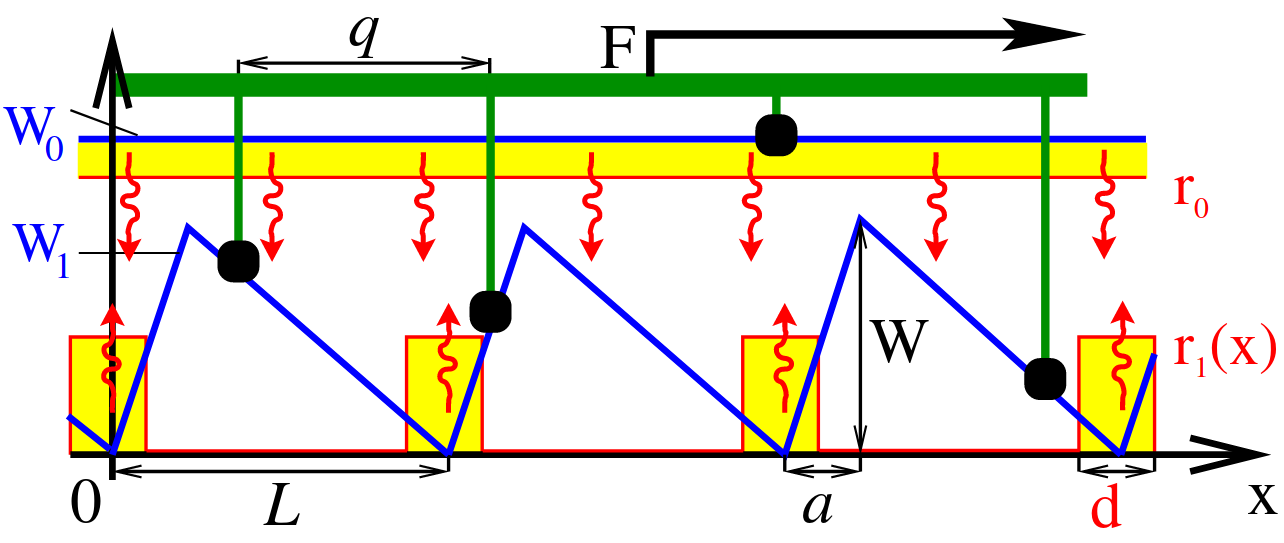
\includegraphics[height=5cm]{coupledmolmot.png}\caption{Gekoppelte molekulare Motoren. Gr"un: Ger"ust mit "aquidistant befestigten Motoren, Blau: zustands-u. ortsabh"angige Potentiale $W_{\sigma_i}$, Gelb: Raten $r_0$(0 $\rightarrow$ 1) und $r_1$(1 $\rightarrow$ 0)}
%\end{figure}
%\end{frame}
%\begin{frame}{Theorie: Bewegungsgleichung}
%\begin{itemize}
%	\item Kraft durch die Motoren:
%	\begin{align*}
%F_{mot}=-\sum_{i=1}^{N}\partial_xW_{\sigma_i}(x_i)
%	\end{align*}
%	\item Bewegungsgleichung des R"uckgrats 
%	\begin{align*}
%\dot{x}=\frac{1}{\lambda}\left[f_{mot}+f_{ext}+\eta(t)\right]
%	\end{align*}
%	mit 
%\begin{align*}
%	f_{mot}&=F_{mot}/N\\
%	f_{ext}&=F_{ext}/N\\ \left<\eta(t)\eta(t')\right>&=(2k_BT\lambda/N)\delta(t-t')
%\end{align*}
%\end{itemize}
%\end{frame}
%\subsection{Simulation}
%\begin{frame}{Simulation mit symmetrischem Potential}
%\begin{tikzpicture}
%\node (img1)[xshift=0cm][yshift=0cm] {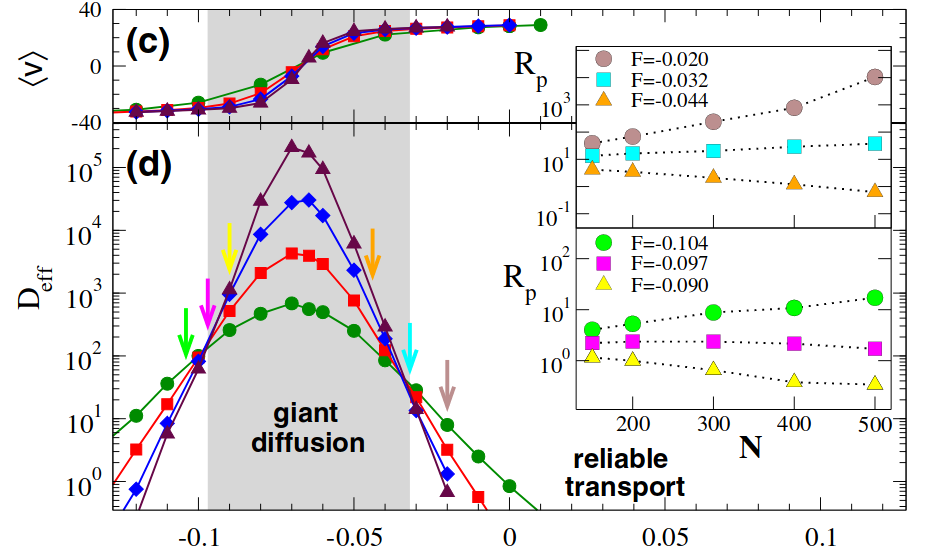
\includegraphics[scale=0.335]{molmotsim2.png}};
%\node (img2) at (img1.north west)[yshift=-3.2cm][xshift=5.62cm] {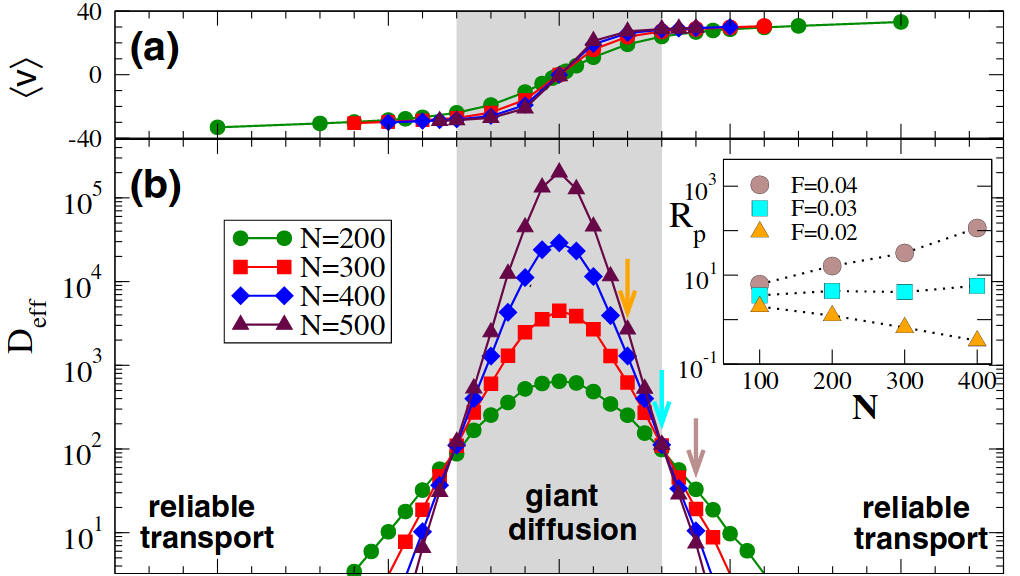
\includegraphics[scale=0.3]{molmotsim1.png}};
%\end{tikzpicture}
%\end{frame}
%\subsection{Simulation}
%\begin{frame}{Simulation mit asymmetrischem Potential}
%\begin{figure}	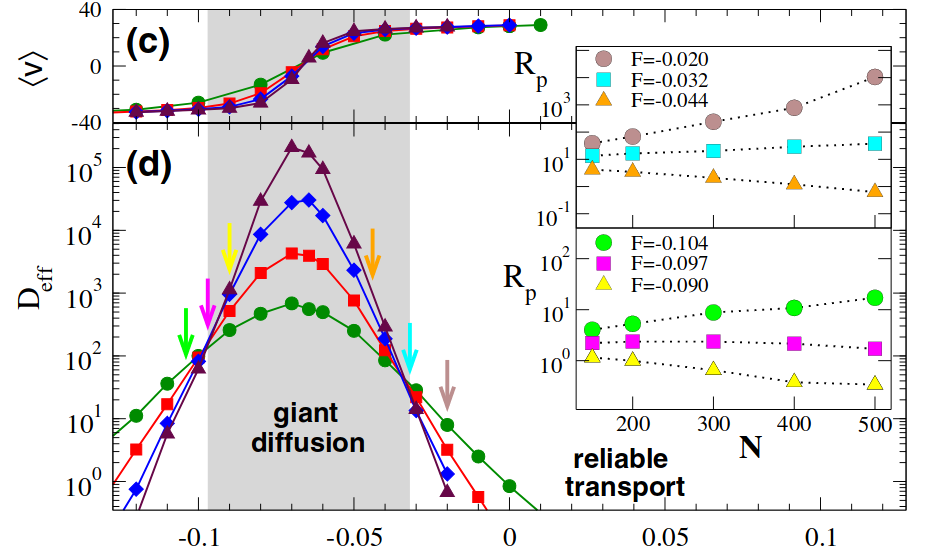
\includegraphics[scale=0.33]{molmotsim2.png}\
%\end{figure}
%\end{frame}
\subsection{Giant diffusion}
%\begin{frame}
%\begin{center}
%	\Huge{\textcolor{darkred}{Brownian}}
%\end{center}
%\begin{center}
%	\Huge{\textcolor{darkred}{particles}}
%\end{center}
%\begin{center}
%	\Huge{\textcolor{darkred}{in a tilted}}
%\end{center}
%\begin{center}
%	\Huge{\textcolor{darkred}{periodic}}
%\end{center}
%\begin{center}
%	\Huge{\textcolor{darkred}{potential}}
%\end{center}
%\end{frame}
%\begin{frame}{Theorie: Bewegungsgleichungen}
%\begin{itemize}
%	\item Langevin-Gleichung:
%	\begin{align*}
%\dot{x}&=v\\
%\dot{v}&=-\gamma v -U'(x)+\sqrt{2\gamma kT}\xi(t)
%	\end{align*}
%	mit\footnotemark[1]
%	\begin{align*}
%U(x)=-Fx-d\cos(x)
%	\end{align*}
%	\item $\gamma$: Reibungskoeffizient, $\left<\xi(t)\xi(t')\right>=\delta(t-t')$, $d=1$
%\end{itemize}
%\footnotetext[1]{Benjamin Lindner und Igor M. Sokolov, "Giant diffusion of underdamped particles in a biased periodic potential," \textit{Physical Review E 93}, 2016.}
%\end{frame}
\begin{frame}{Giant diffusion of Brownian particles\footnotemark[1]}
\begin{columns}[t]
	\column{.5\textwidth}
	\centering
	\vspace{-0.5cm}
\begin{figure}	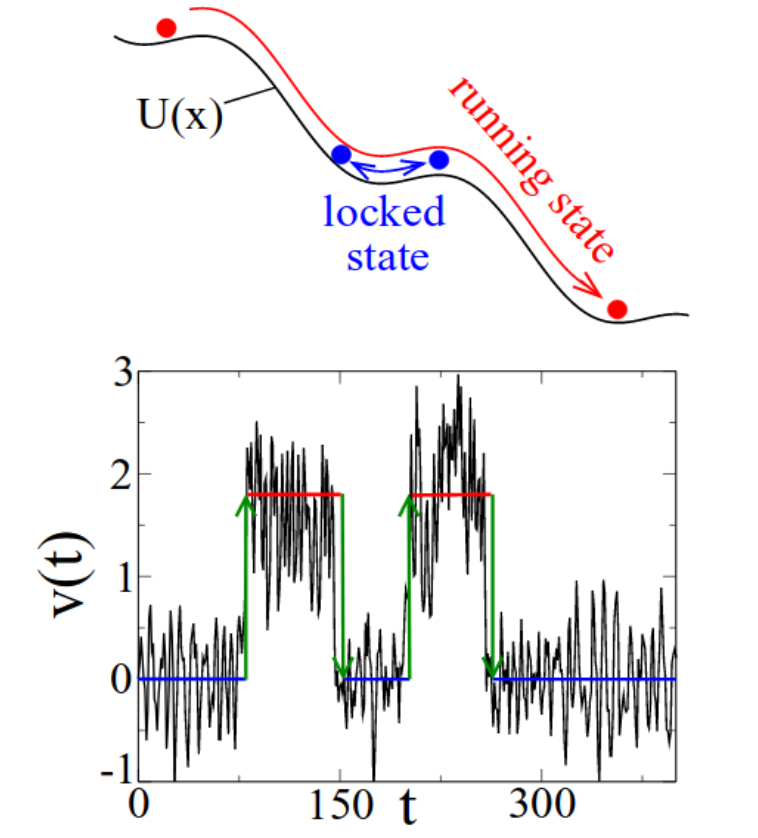
\includegraphics[scale=0.28]{nbpveldyncor2.png}\
\end{figure}
	\column{.5\textwidth}
	\begin{itemize}
		\item Motion of particles in a tilted cosine potential
	\end{itemize}
\bigskip\bigskip\bigskip\bigskip
\begin{itemize}
	\item \textbf{bistability} of velocity
	\item effective diffusion coefficient:
	\begin{align*}
		D_{eff}=lim_{t\rightarrow\infty}\frac{\left\langle x^2(t) \right\rangle-\left\langle x(t)\right\rangle ^2}{2t}
		\end{align*}
\end{itemize}
\end{columns}
\footnotetext[1]{B. Lindner and I. M. Sokolov, "Giant diffusion of underdamped particles in a biased periodic potential", \textit{PRE 93}, 2016.}
\end{frame}
\begin{frame}{Giant diffusion of Brownian particles}
\begin{figure}	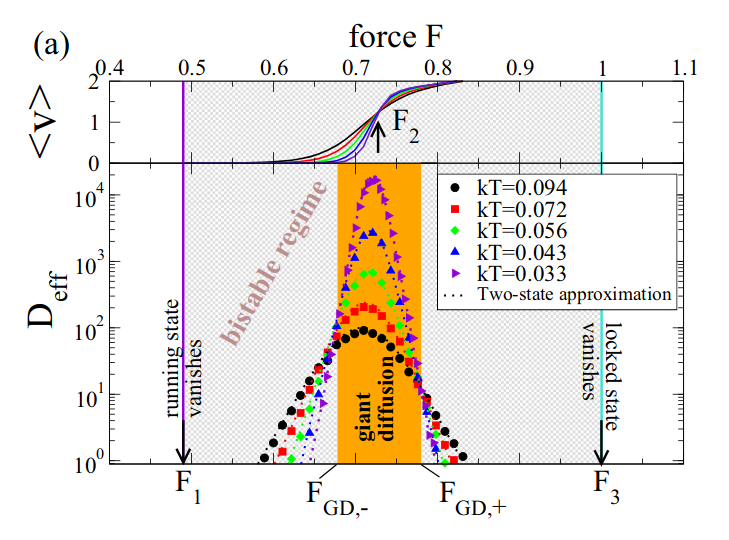
\includegraphics[scale=0.4]{nbpsim1.png}\
\end{figure}
\end{frame}
%\begin{frame}{Simulation - kritischer Bereich}
%\begin{figure}	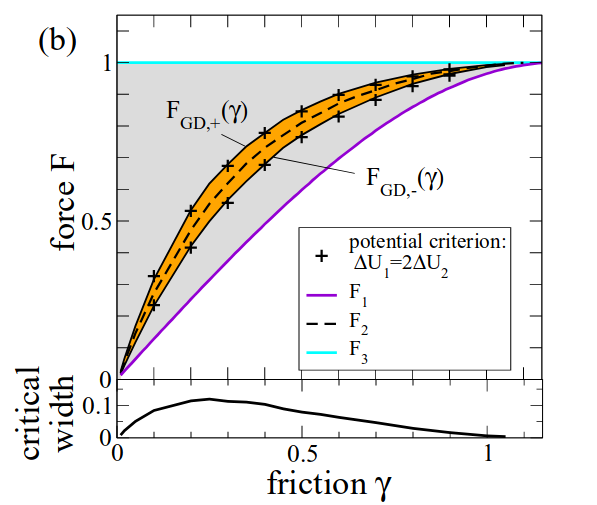
\includegraphics[scale=0.4]{nbpsim2.png}\
%\end{figure}
%\end{frame}
%\subsection{Auswertung}
%\begin{frame}{Berechnung effektiver Potentialbarrieren}
%\begin{itemize}
%	\item Annahme: "Ubergangsraten zeigen Kramers-"ahnliches Verhalten:
%	\begin{align*}
%w\propto T^\alpha \text{e}^{-\frac{\Delta U}{kT}}
%	\end{align*}
%
%	\begin{figure}	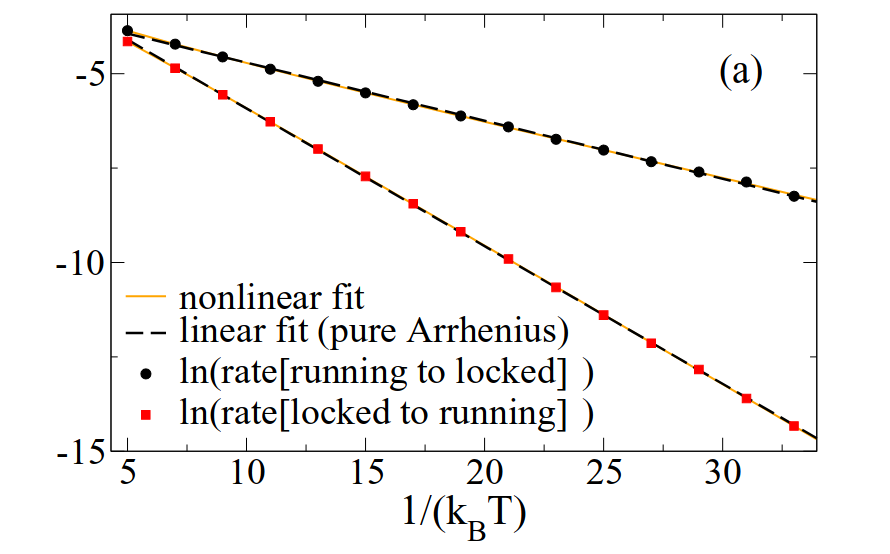
\includegraphics[scale=0.25]{kramerfit.png}\
%	\end{figure}	
%\item Fits f"ur $\alpha=0$ und $\alpha \neq 0$ liefern "ahnliche Barrieren
%	\end{itemize}
%\end{frame}

%\begin{frame}{Berechnung effektiver Potentialbarrieren}
%\begin{itemize}
%	\item Plotten von $\Delta U$ und $2\Delta U$ f"ur verschiedene Kr"afte 
%	\begin{figure}	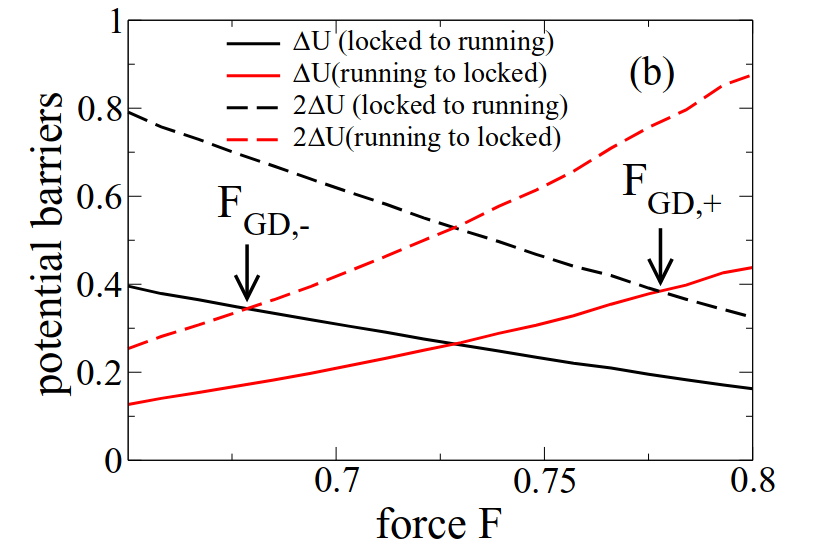
\includegraphics[scale=0.25]{barrierplot.png}\
%	\end{figure}	
%	\item Schnittpunkte etwa bei $F=0.68$ und $F=0.78$ 
%\end{itemize}
%\end{frame}
%\begin{frame}{Berechnung effektiver Potentialbarrieren}
%\begin{itemize}
%	\item Vergleich mit Simulation
%	\begin{figure}	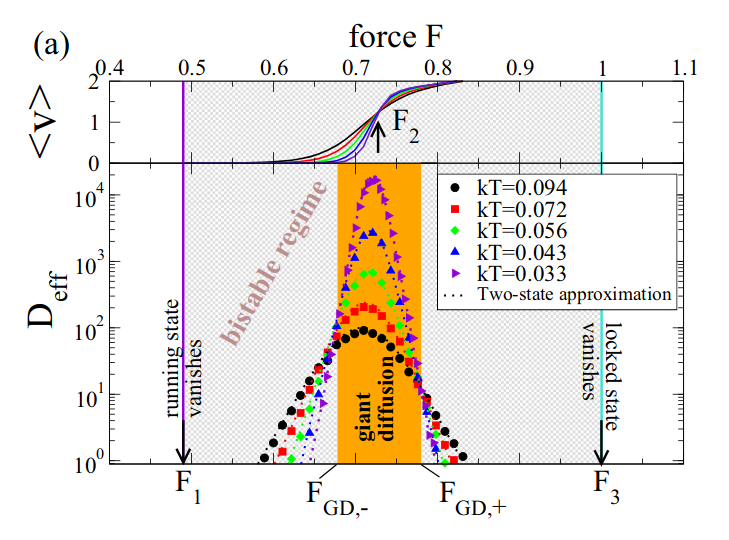
\includegraphics[scale=0.37]{nbpsim1.png}\
%	\end{figure}	
%\end{itemize}
%\end{frame}
%\subsection{Reproduktion}
%\begin{frame}{Reproduktion: Geschwindigkeit}
%\begin{figure}	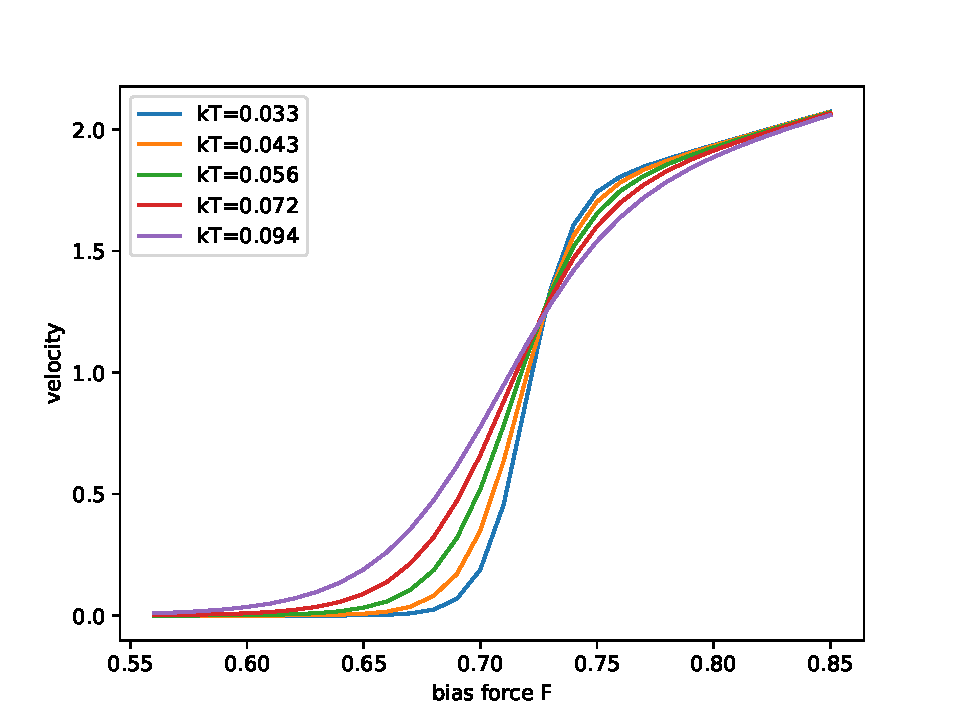
\includegraphics[scale=0.6]{gmechexaktnew.pdf}\
%\end{figure}
%\end{frame}
%\begin{frame}{Reproduktion: Diffusionskoeffizient}
%\begin{figure}	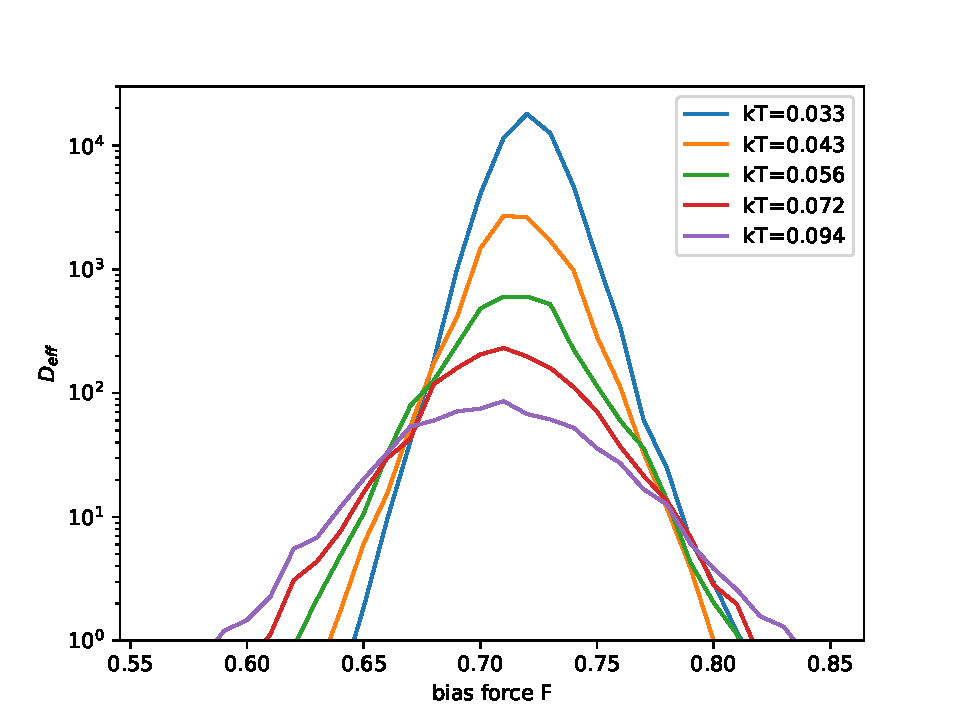
\includegraphics[scale=0.6]{dmechexaktnew.pdf}\
%\end{figure}
%\end{frame}
%\begin{frame}{Reproduktion: Fano - Faktor}
%\begin{figure}	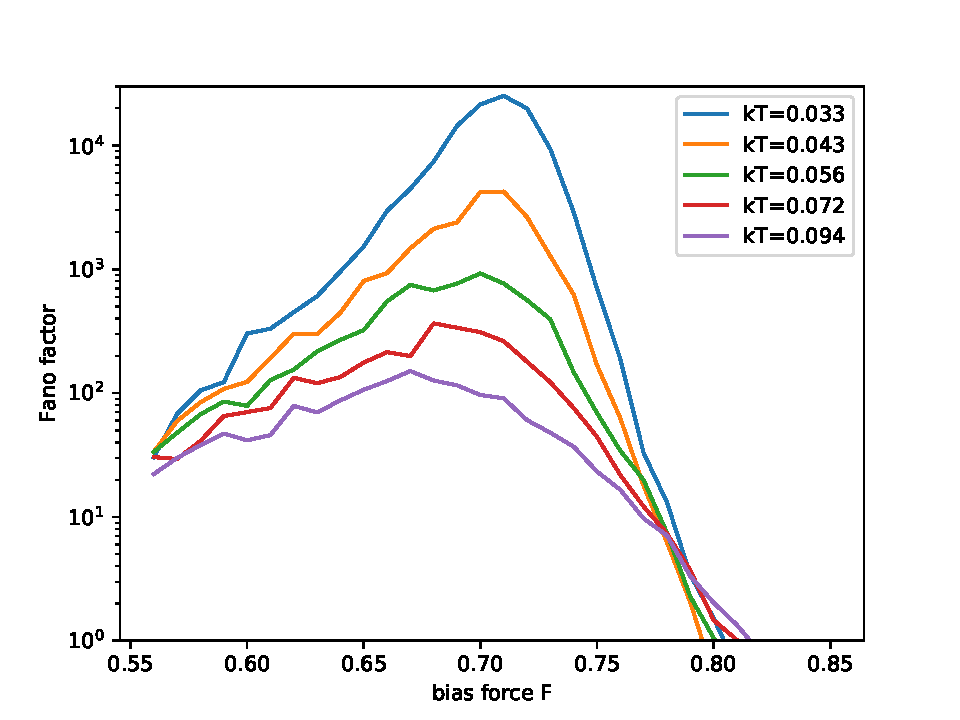
\includegraphics[scale=0.6]{fmechexaktnew.pdf}\
%\end{figure}
%\end{frame}

\subsection{Transition to Neuron models}
%\begin{frame}
%\begin{center}
%	\Huge{\textcolor{darkred}{Neuron models}}
%\end{center}

%\end{frame}
\begin{frame}{Brownian particle vs Neuron model}
\begin{figure}	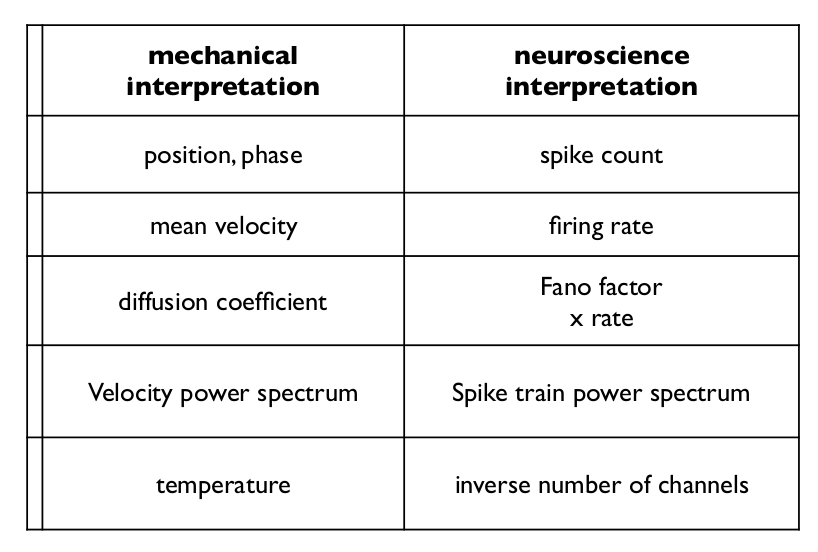
\includegraphics[scale=0.4]{ubergang.png}
\end{figure}
\end{frame}
\begin{frame}{Quantities of interest in neuron models}
\begin{itemize}
	%\item station"are L"osung $\left(\text{mit} -U'(v)=f(v)/g^2(v)\right)$:
	%\begin{equation}\nonumber
	%P_0(v)=\frac{\text{e}^{-U(v)/Q}/g^2(v)}{|| \cdot ||}
	%\end{equation}
	\item effective diffusion coefficient
	\begin{align*}
		D_{eff}=lim_{t\rightarrow\infty}\frac{\left\langle x^2(t) \right\rangle-\left\langle x(t)\right\rangle ^2}{2t}=\frac{\left\langle N^2(t) \right\rangle-\left\langle N(t)\right\rangle ^2}{2t}
		\end{align*}
	\item mean velocity (firing rate):
	\begin{align*}
	r =lim_{t\rightarrow\infty}\frac{\left\langle x(t)-x(0) \right\rangle}{t}=\frac{\left\langle N(t) \right\rangle}{t}
	\end{align*}
	
	\item Fano factor:
	\begin{align*}
	F=\frac{\left\langle \Delta N^2(t) \right\rangle}{\left\langle N(t)\right\rangle}
	\end{align*}
\end{itemize}
\end{frame}
\subsection{Goals}
\begin{frame}{Goals of this thesis}
\begin{itemize}
	\setlength\itemsep{2em}
	\item Primary goal: induce stochastic \textbf{bursting} in \textbf{simple} neuron models and investigate spike count statistics
	\item find \textbf{critical points} where firing pattern changes drastically
	\item Secondary goal: simulate neurons under influence of periodic stimulus to explore \textbf{signal transmission}
\end{itemize}
\end{frame}

%\begin{frame}
%\begin{center}
%	\Huge{\textcolor{darkred}{$I_{Na,p}+I_K$ Modell}}
%\end{center}
%\begin{center}
%	\Huge{\textcolor{darkred}{mit}}
%\end{center}
%\begin{center}
%	\Huge{\textcolor{darkred}{Sattel-Knoten-}}
%\end{center}
%\begin{center}
%	\Huge{\textcolor{darkred}{Bifurkation}}
%\end{center}
%\end{frame}
%\section{$I_{Na,p}+I_K$-Modell mit Sattel-Knoten Bifurkation}

%\subsection{Bistabilit"at}
%
%\begin{frame}{Phasenraum}
%\begin{columns}[t]
%	\column{.5\textwidth}
%	\centering
%	\vspace{-1cm}
%	\begin{figure}
%		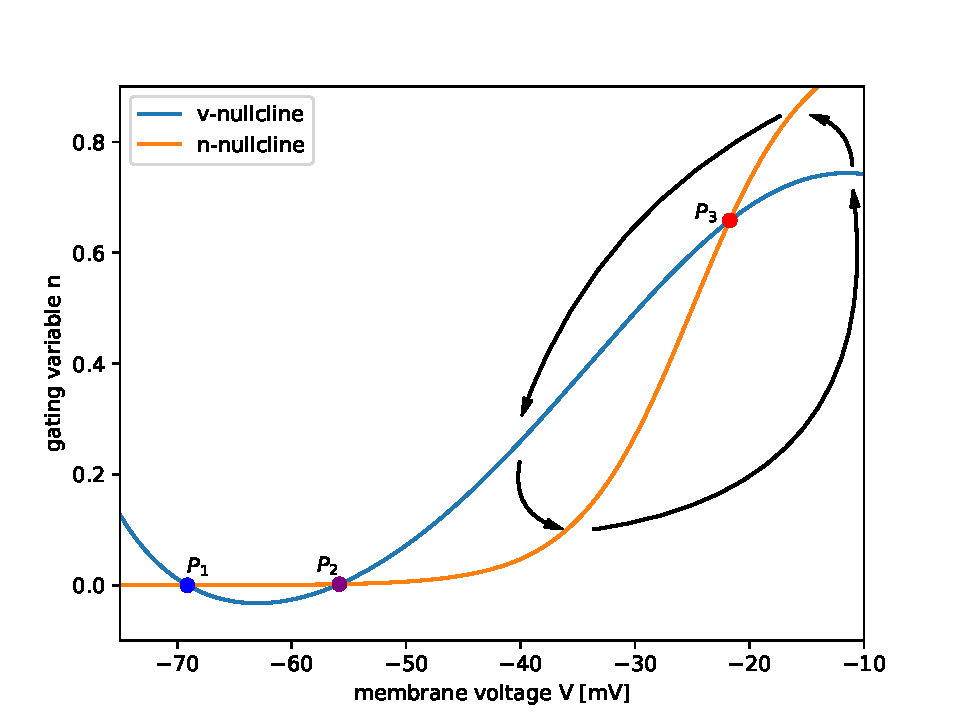
\includegraphics[scale=0.3]{Isoklinen.pdf}
%	\end{figure}
%	\vspace{-0.5cm}
%	\begin{figure}
%		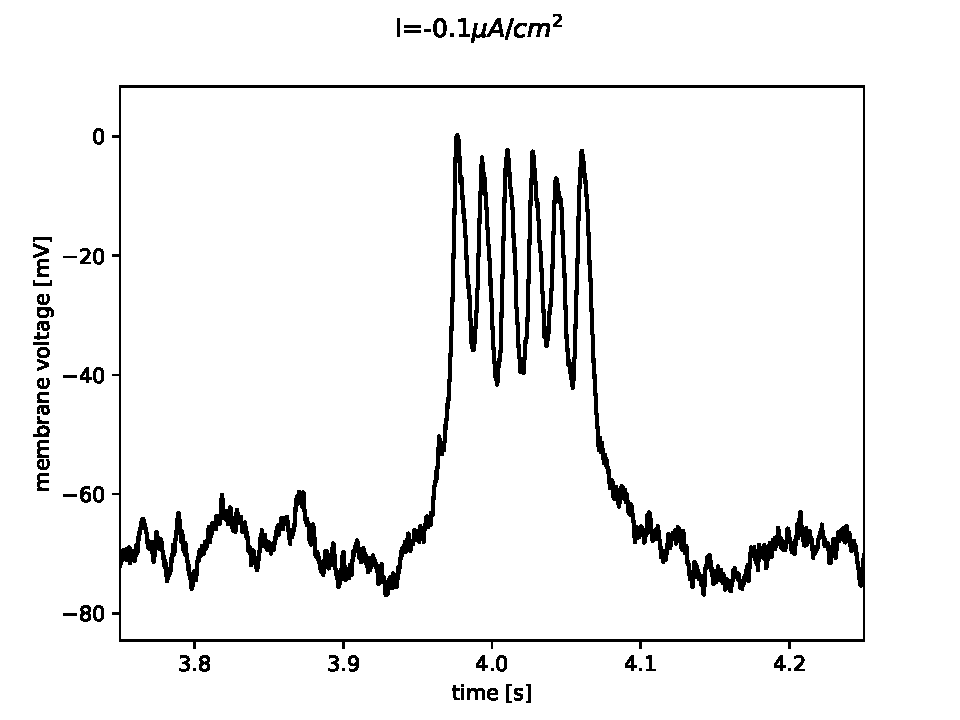
\includegraphics[scale=0.3]{V-t-diagramm.pdf}
%	\end{figure}
%	\column{.5\textwidth}
%	\centering
%	\vspace{-1cm}
%	\begin{figure}
%		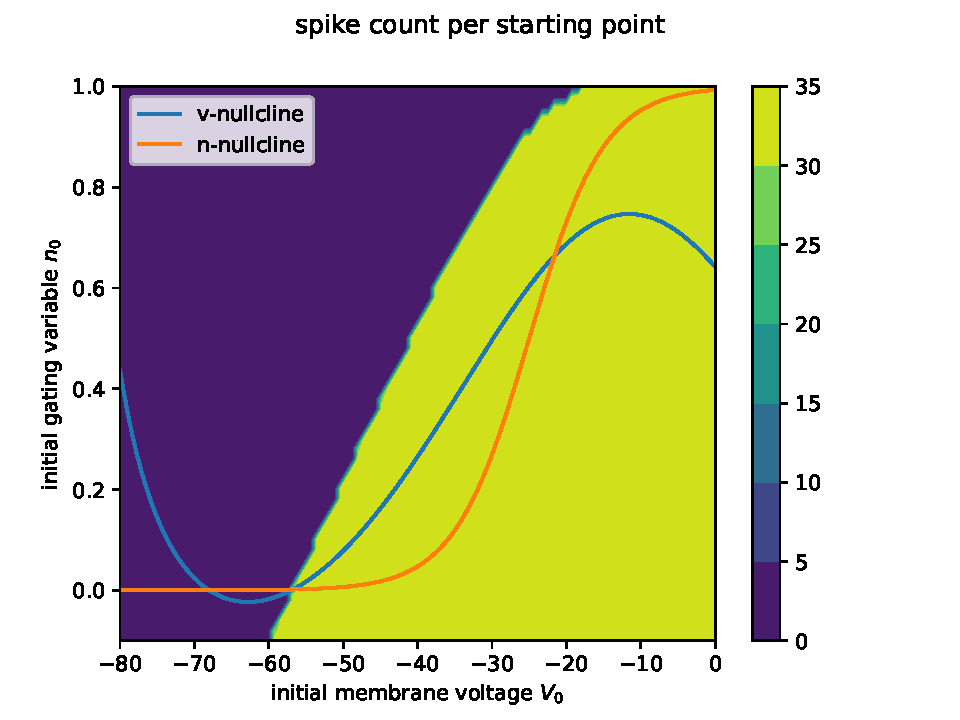
\includegraphics[scale=0.3]{Startparam_lang.pdf}
%	\end{figure}\vspace{-0.7cm}
%	\begin{figure}
%		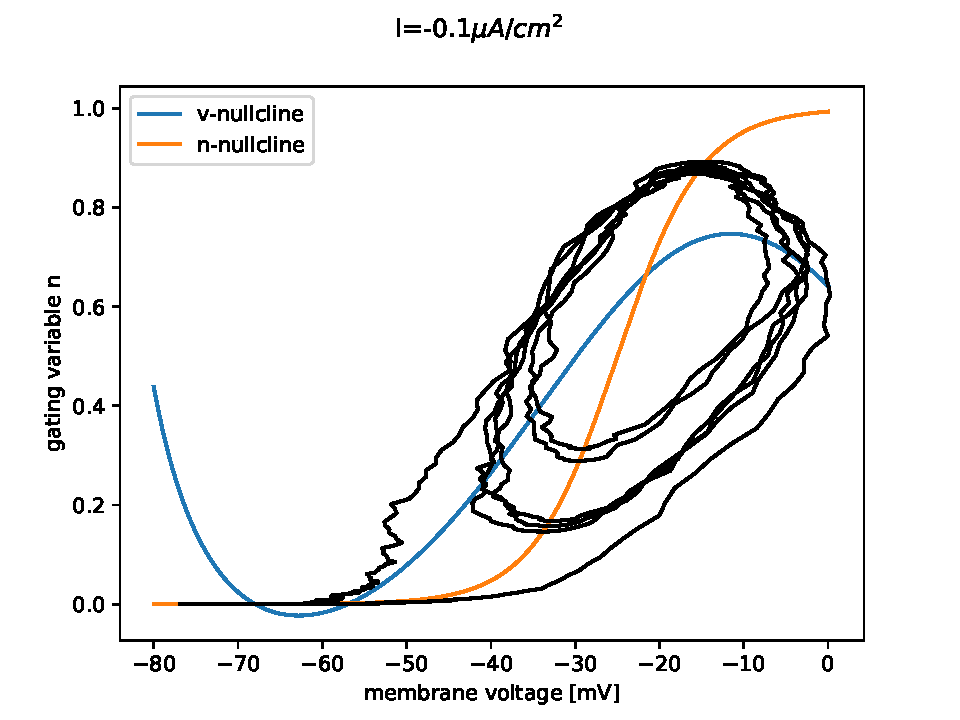
\includegraphics[scale=0.3]{n-V-diagramm.pdf}
%	\end{figure}
%	%\begin{itemize}
%	%	\item links oben: rauschinduzierte "Uberg"ange bei $I=0$
%	%	\item rechts oben: I=1
%	%	\item links unten: I=3
%	%\end{itemize}
%\end{columns}
%\end{frame}
%\begin{frame}{Variation von $I$}
%\begin{columns}[t]
%	\column{.5\textwidth}
%	\centering
%	\vspace{-1cm}
%	\begin{figure}
%		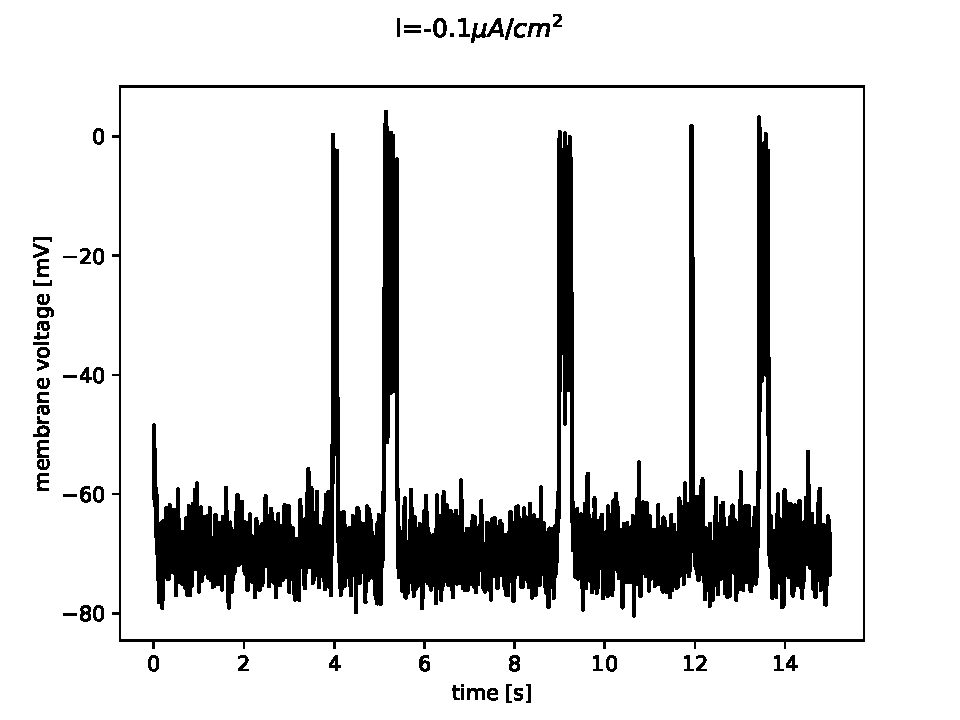
\includegraphics[scale=0.3]{uebergaengeI=-0,1.pdf}
%	\end{figure}
%\vspace{-1cm}
%	\begin{figure}
%	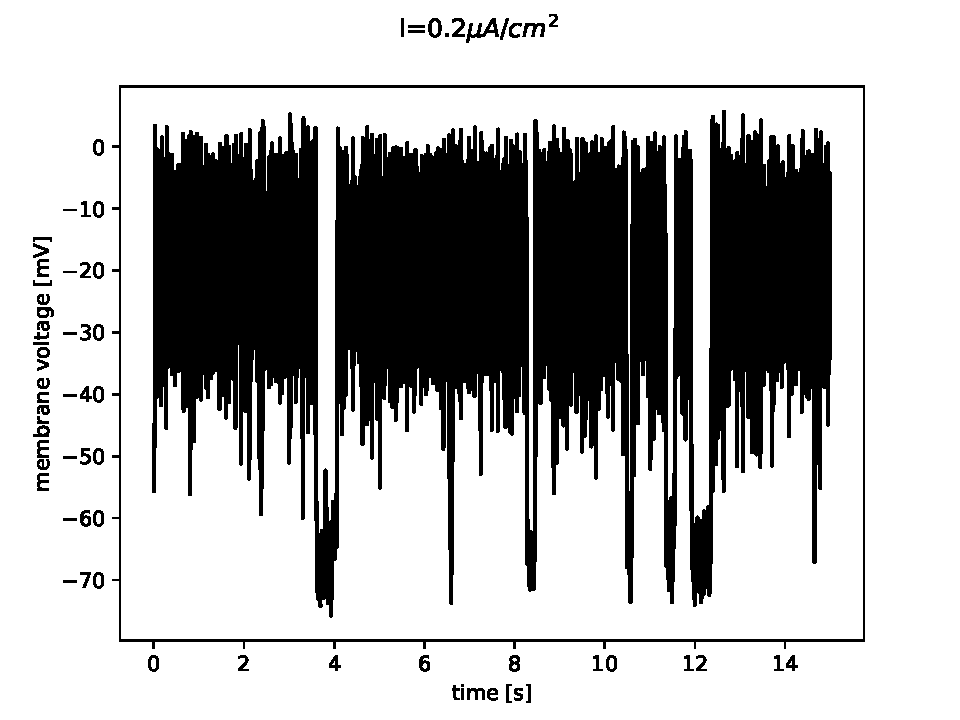
\includegraphics[scale=0.3]{uebergaengeI=0,2.pdf}
%\end{figure}
%	\column{.5\textwidth}
%	\centering
%	\vspace{-0.5cm}
%	\begin{figure}
%		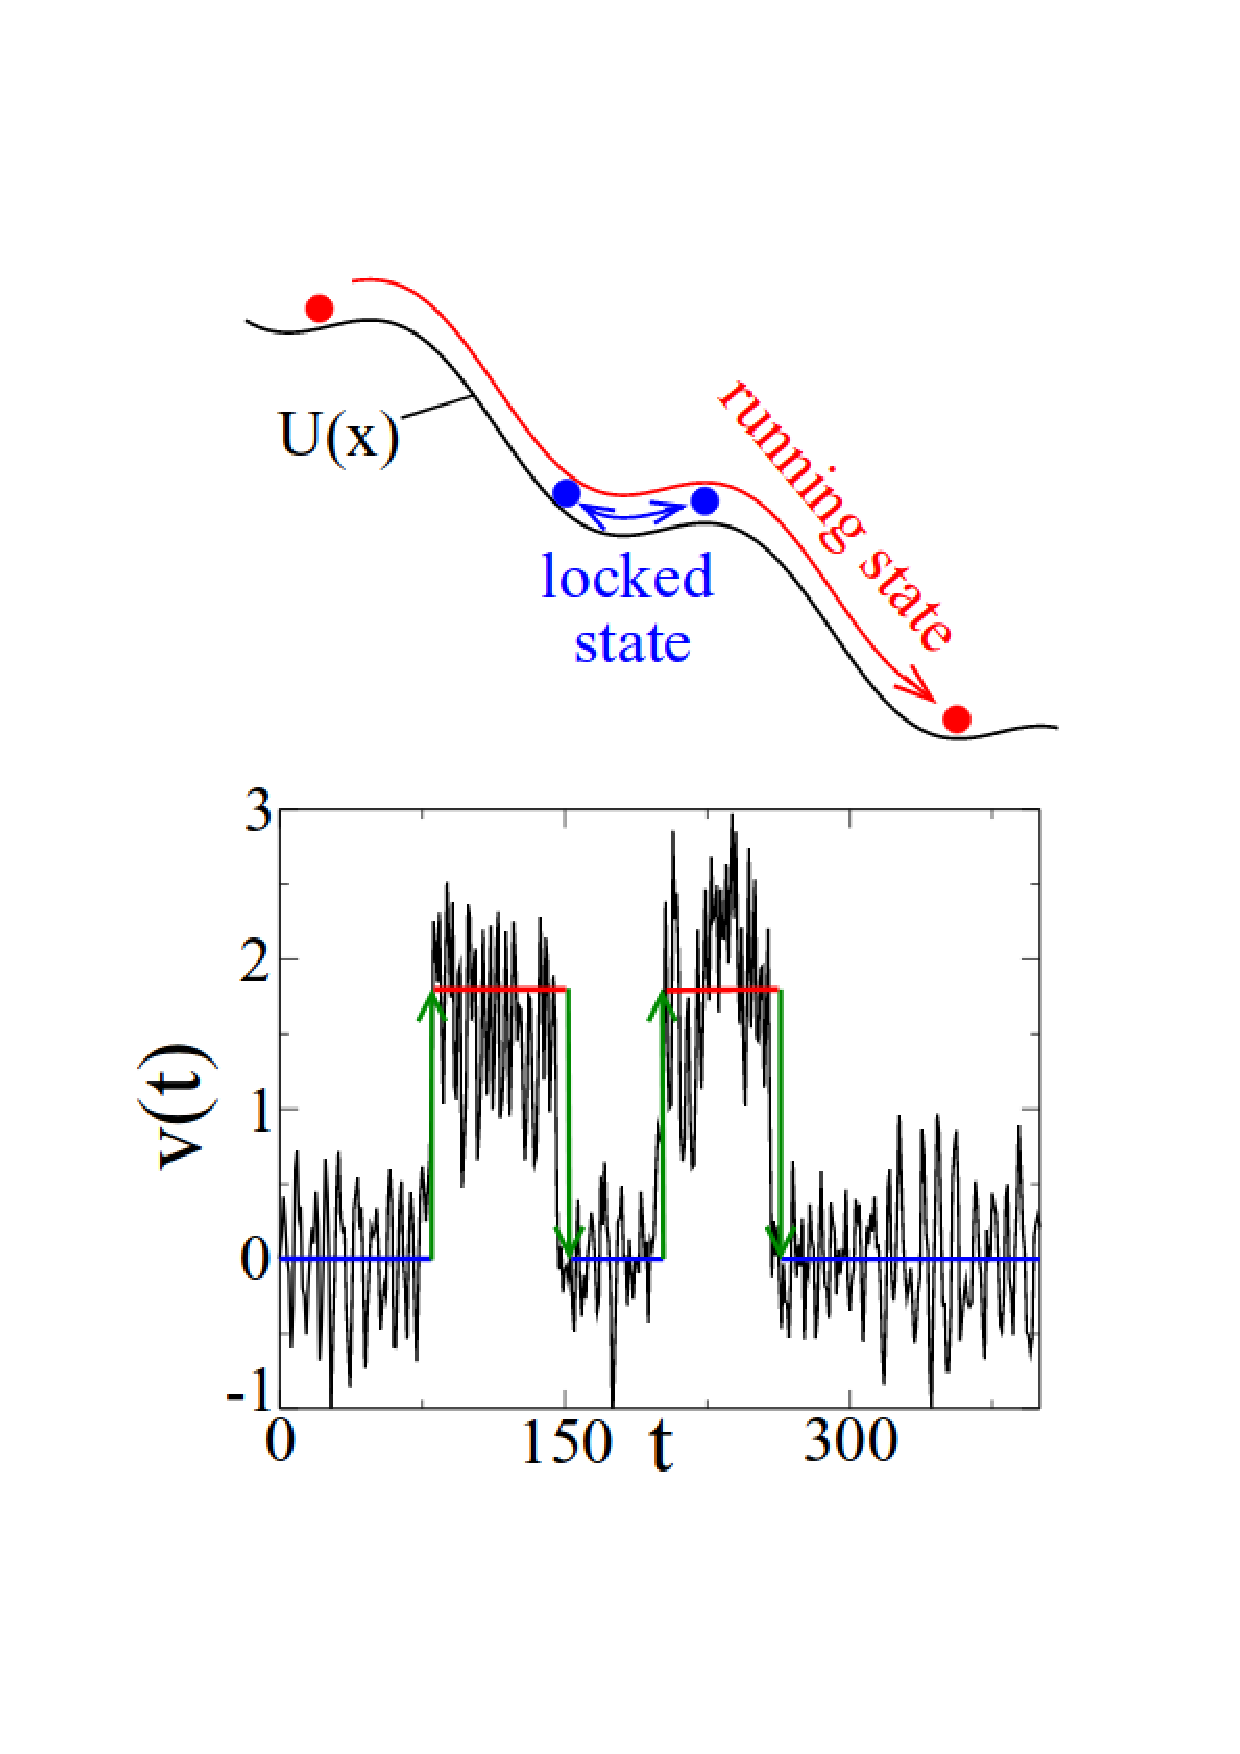
\includegraphics[scale=0.25]{nbpveldyncor.pdf}
%	\end{figure}\vspace{-8.6cm}
%	\begin{figure}
%	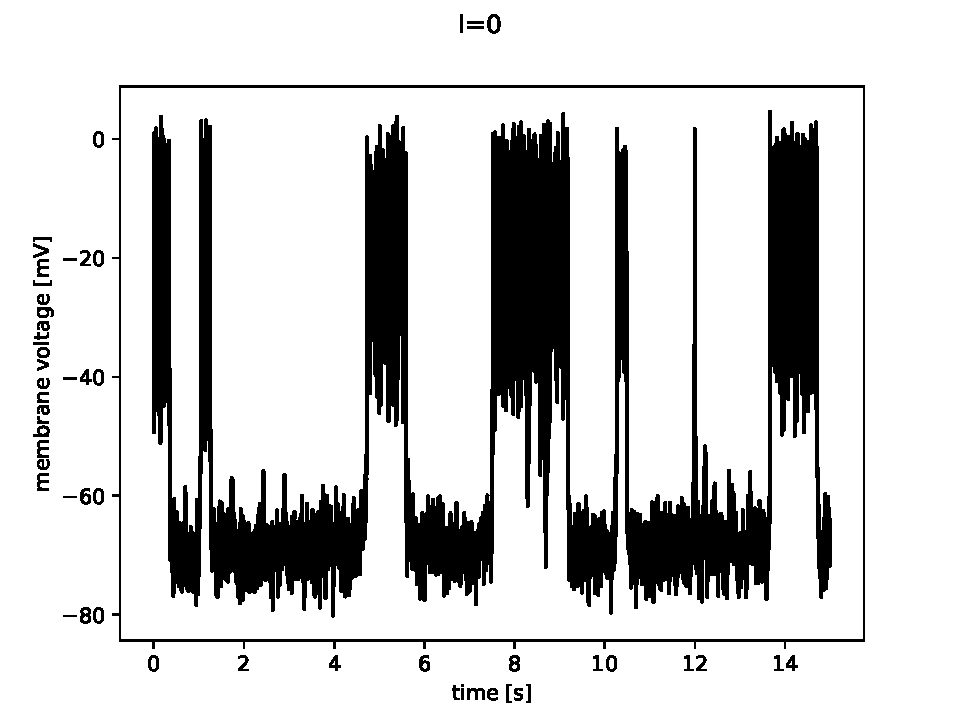
\includegraphics[scale=0.3]{uebergaengeI=0.pdf}
%\end{figure}
%\end{columns}
%\end{frame}
%\subsection{Simulation}
%\begin{frame}{Simulation: Feuerrate}
%	\begin{figure}	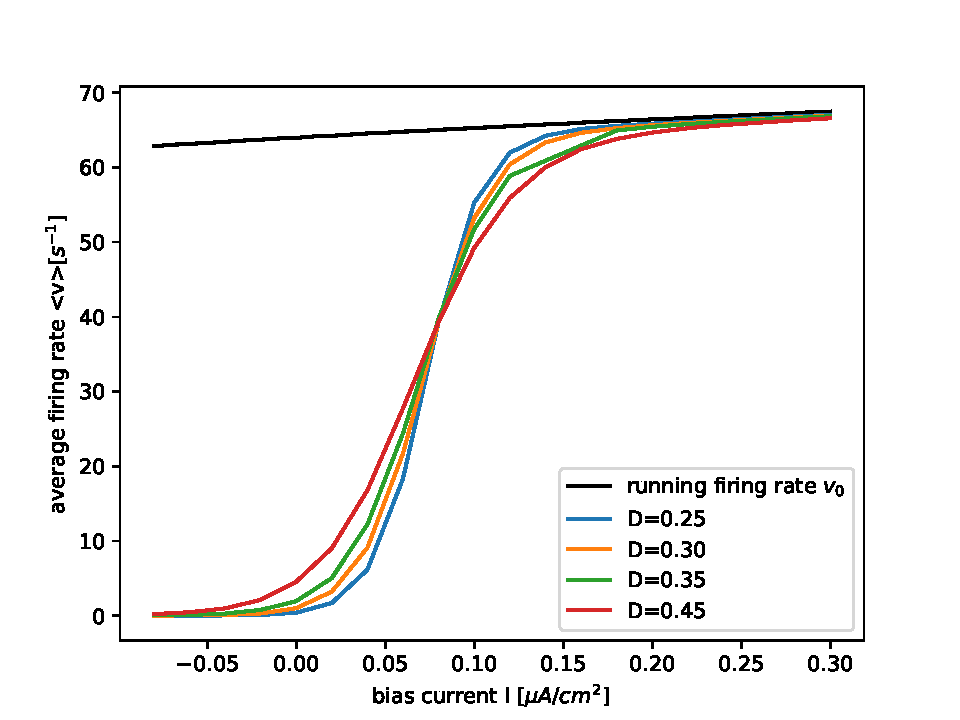
\includegraphics[scale=0.6]{gneur23critrealfast16alcoarsewstfrealfast9acoarsetf.pdf}
%\end{figure}
%\end{frame}
%\begin{frame}{Simulation: Diffusionskoeffizient}
%\begin{figure}	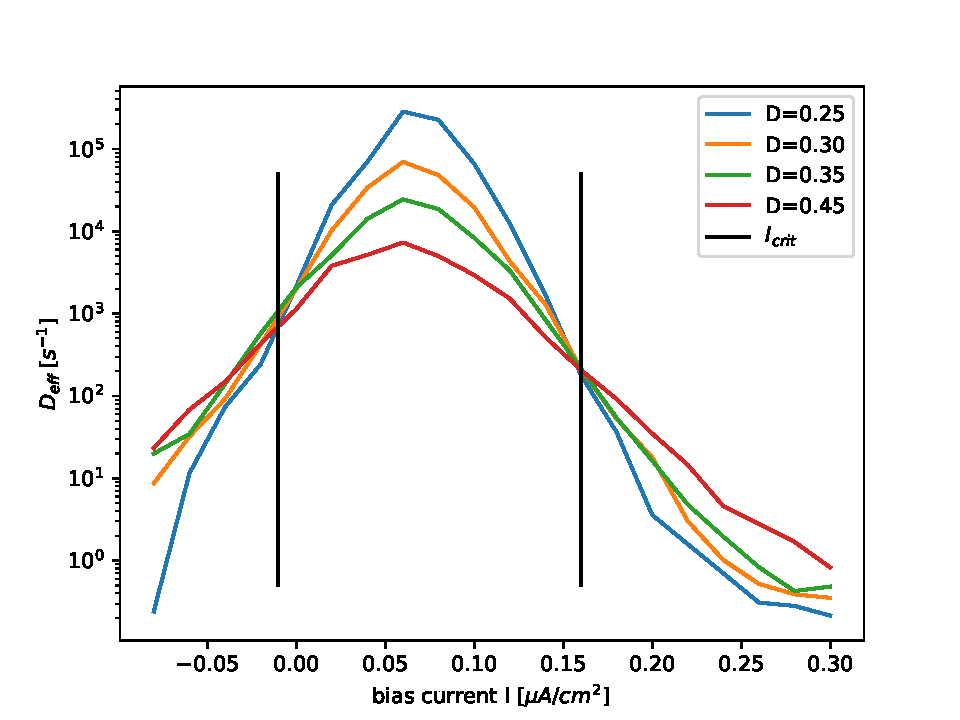
\includegraphics[scale=0.6]{dneur23critrealfast16alcoarsewstfrealfast9acoarsetf.pdf}
%\end{figure}
%\end{frame}
%\begin{frame}{Simulation: Fano-Faktor}
%\begin{figure}	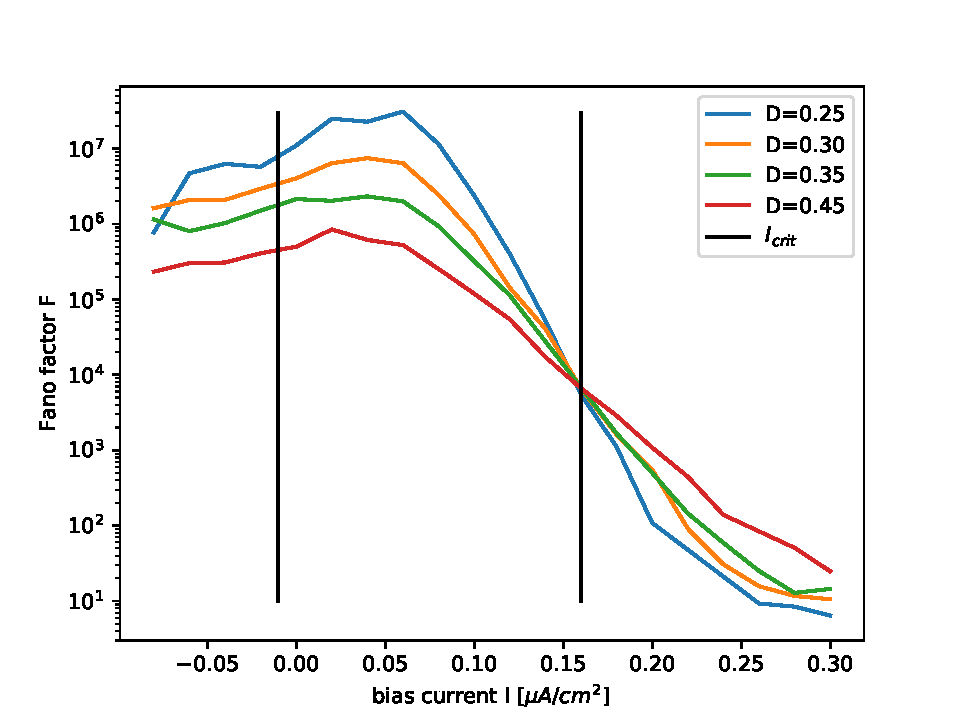
\includegraphics[scale=0.6]{fneur23critrealfast16alcoarsewstfrealfast9acoarsetf.pdf}
%\end{figure}
%\end{frame}
%\begin{frame}{Intervallstatistik}
%\begin{figure}	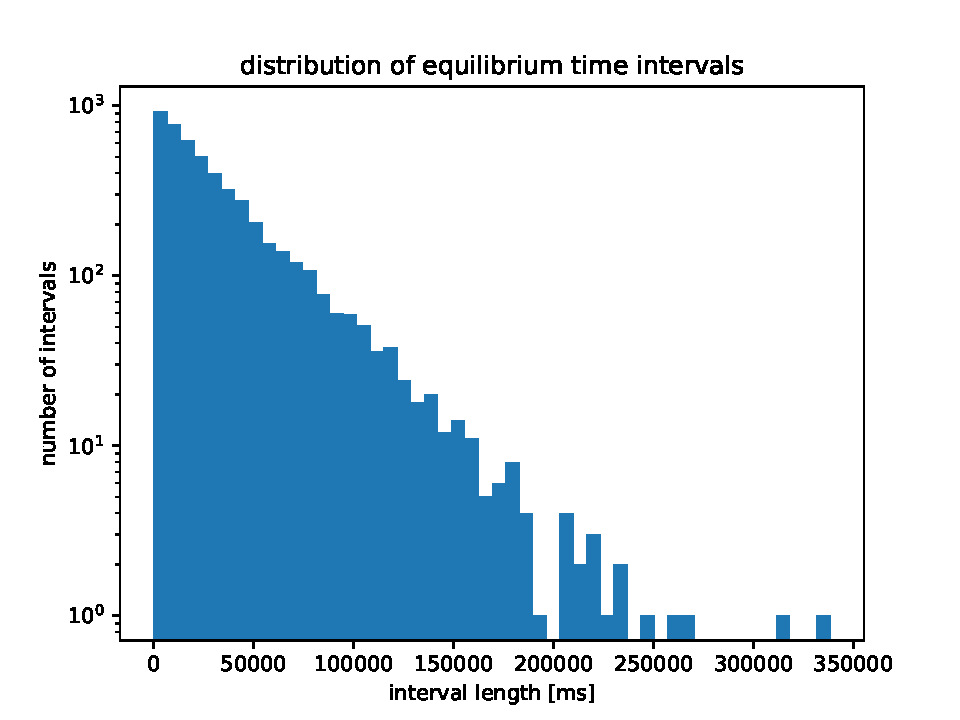
\includegraphics[scale=0.6]{eqdistajrj2newrealfast11jjem2sh359.pdf}
%\end{figure}
%\end{frame}
%\begin{frame}{Arrhenius-Fit}
%\begin{figure}	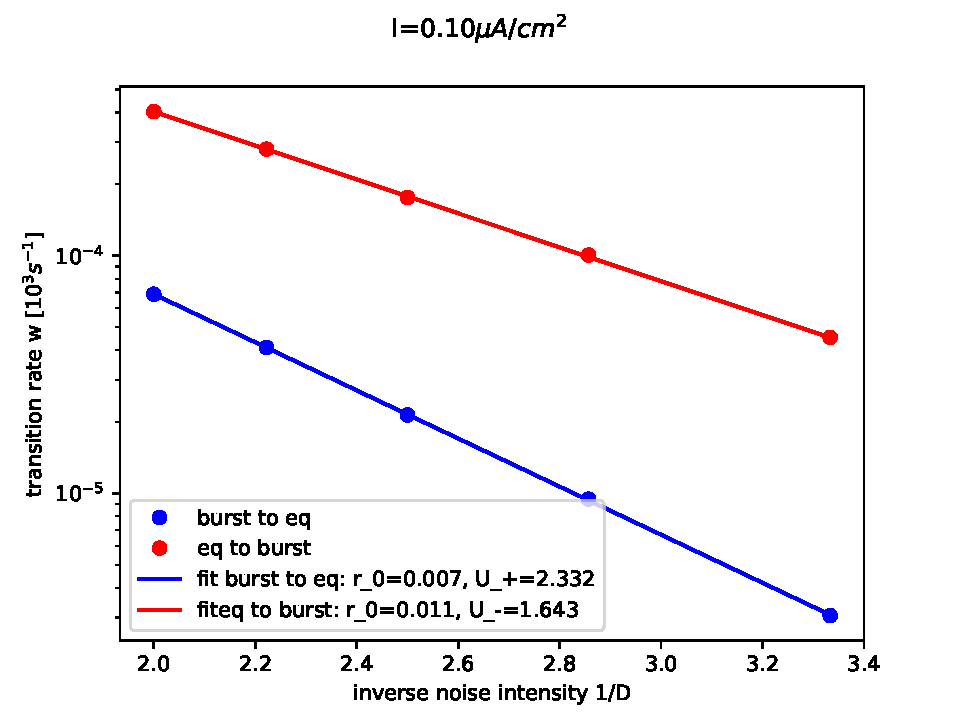
\includegraphics[scale=0.6]{ArrheniusI=0,1.pdf}
%\end{figure}
%\end{frame}
%
%\begin{frame}{Arrhenius-Fit}
%\begin{itemize}
%	\item "Ubergangsraten:
%\begin{align*}
%w_{\pm}=w_{0,\pm}\text{e}^{-\frac{\Delta U_{\pm}}{Q}}
%\end{align*}
%\item $w_{0,\pm}$ und $\Delta U_\pm$ aus Fits:
%\item $D_{\text{eff}}$ und $F$ aus Raten und $\Delta r=r_+-r_-=r_+$:
%\end{itemize}
%\begin{align*}
%D_{\text{eff}}&=\frac{r_+^2 w_+w_-}{(w_++w_-)^3}\\
%F&=\frac{2r_+w_+}{(w_++w_-)^2}
%\end{align*}
%\end{frame}
%\begin{frame}{Barrieren f"ur verschiedene Str"ome}
%\begin{figure}	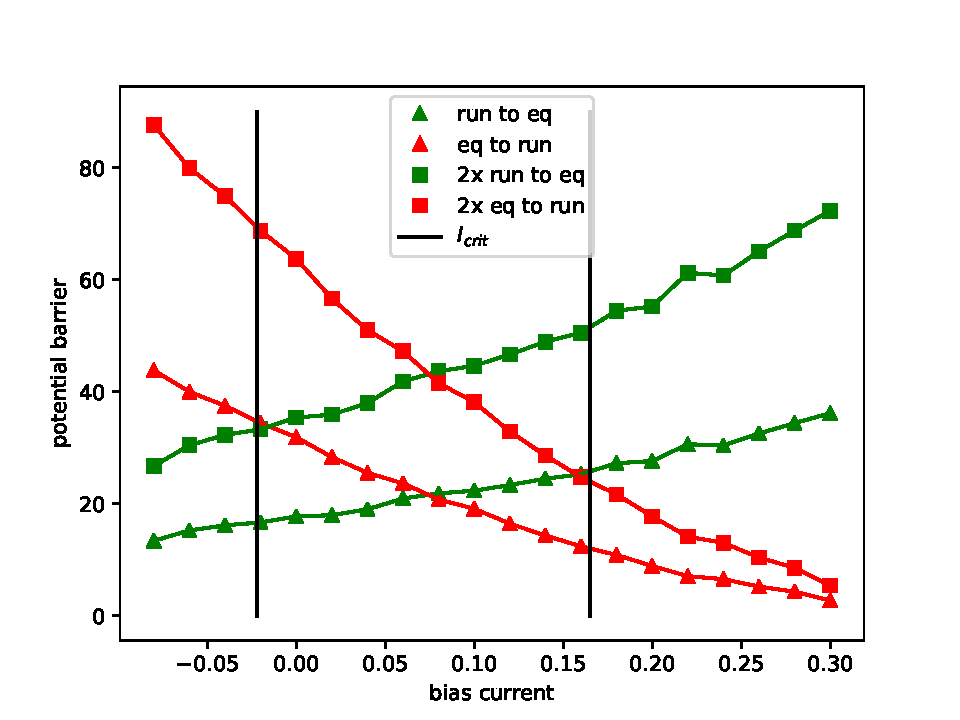
\includegraphics[scale=0.6]{barriercomprealfit4linecrit.pdf}
%\end{figure}
%\end{frame}
%\begin{frame}{Vergleich mit Zwei-Zustands-Modell: $D_{eff}$}
%\begin{figure}	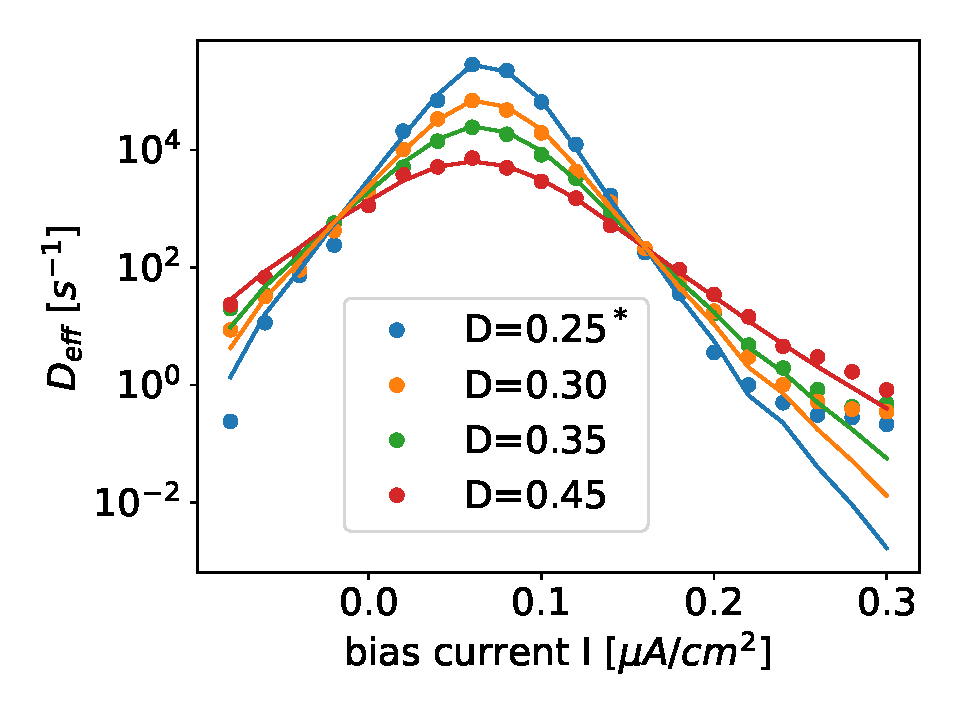
\includegraphics[scale=0.6]{dcompdfpwnewbigrealfast23mtfrealfast19mtf.pdf}
%\end{figure}
%\end{frame}
%\begin{frame}{Vergleich mit Zwei-Zustands-Modell: $F$}
%\begin{figure}	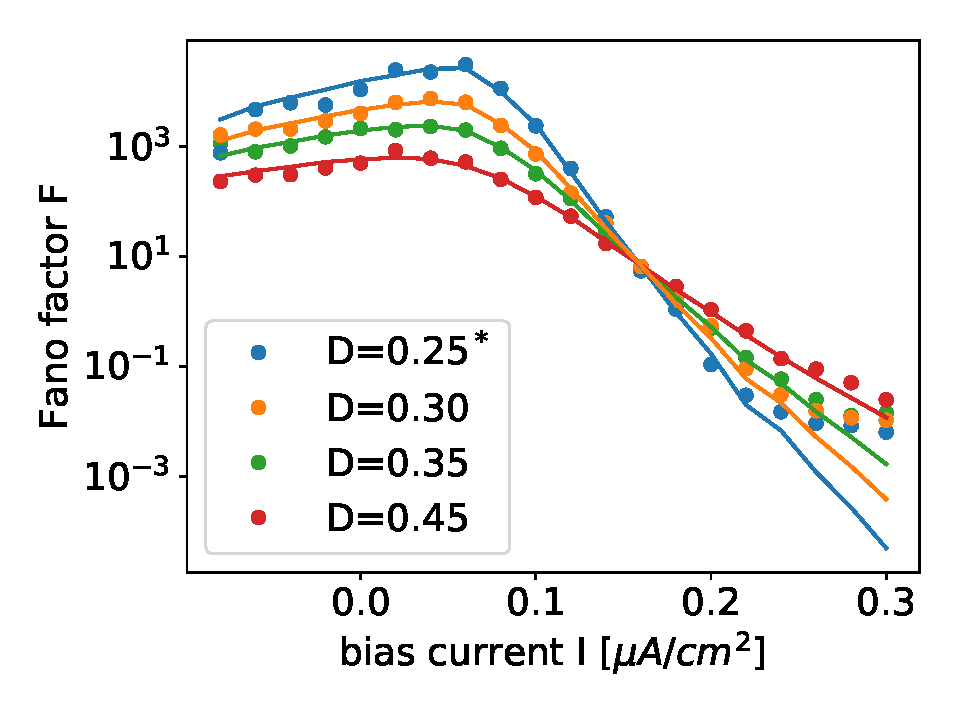
\includegraphics[scale=0.6]{fcompdfpwnewbigrealfast23mtfrealfast19mtf.pdf}
%\end{figure}
%\end{frame}
%\begin{frame}{Vorhersage des Zwei-Zustands-Modells}
%\begin{figure}	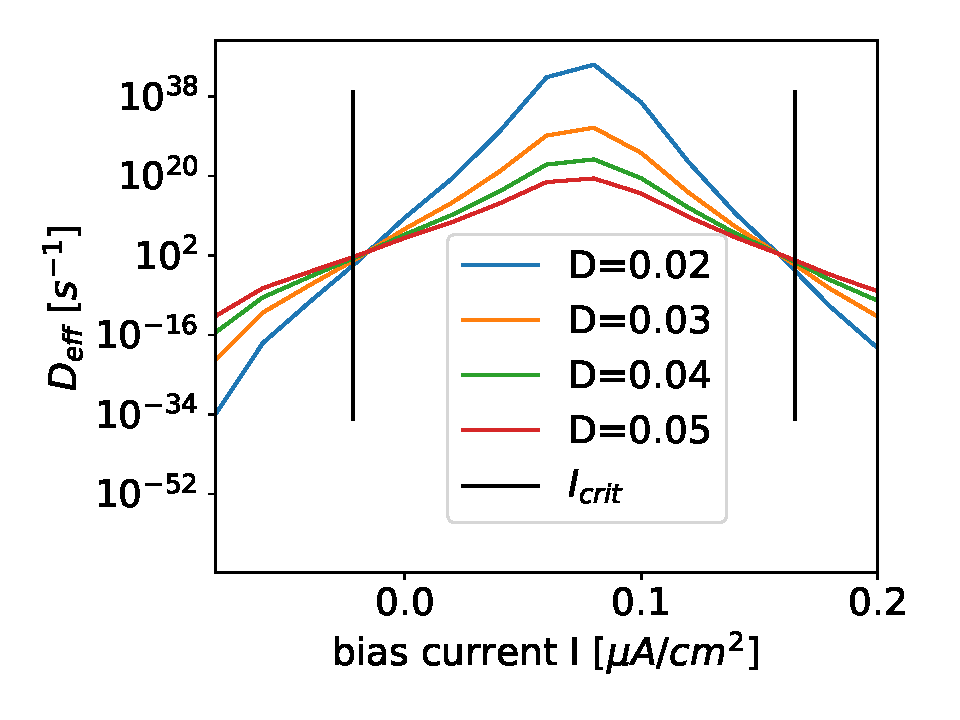
\includegraphics[scale=0.6]{dcompdfpwnewpred2realfast11jjem2shrealfast19jjem2st.pdf}
%\end{figure}
%\end{frame}
\section{$I_{Na,p}+I_K$ model with Andronov-Hopf bifurcation}
%\begin{frame}
%\begin{center}
%	\Huge{\textcolor{darkred}{$I_{Na,p}+I_K$ model}}
%\end{center}
%\begin{center}
%	\Huge{\textcolor{darkred}{with}}
%\end{center}
%\begin{center}
%	\Huge{\textcolor{darkred}{Andronov-Hopf-}}
%\end{center}
%\begin{center}
%	\Huge{\textcolor{darkred}{bifurcation}}
%\end{center}
%\end{frame}
\subsection{Theory}
\begin{frame}{Model}
\begin{adjustwidth}{-1em}{-1em}
	\begin{itemize}
		\item $I_{Na,p}+I_K$ model:
		\begin{align*}
		C\dot{V} &= I - g_L(V-E_L) - g_{Na}m_{\infty}(V)(V-E_{Na}) - g_Kn(V-E_K)+\sqrt{2D}\xi(t)\\
		\dot{n} &= (n_{\infty}(V)-n)/\tau(V)
		\end{align*}
		%\item Steady-State-Aktivierungsfunktion:
		%\begin{align*}
		%f_{\infty}(V) = \frac{1}{1+\exp\{(V_{1/2}-V)/k\}}
		%\end{align*}
		%\item hierbei ist k die Steigung, sowie:
		%\begin{align*}
		%f_{\infty}(V_{1/2})=1/2
		%\end{align*}
		\begin{columns}[t]
			\column{.55\textwidth}
			Steady-State activation function:
			\begin{align*}
			f_{\infty}(V) = \frac{1}{1+\exp\{(V_{1/2}-V)/k\}}
			\end{align*}
			where k is the slope factor and
			\begin{align*}
			f_{\infty}(V_{1/2})=1/2
			\end{align*}
			\column{.45\textwidth}
			\centering
			\vspace{-1cm}
			\begin{figure}
				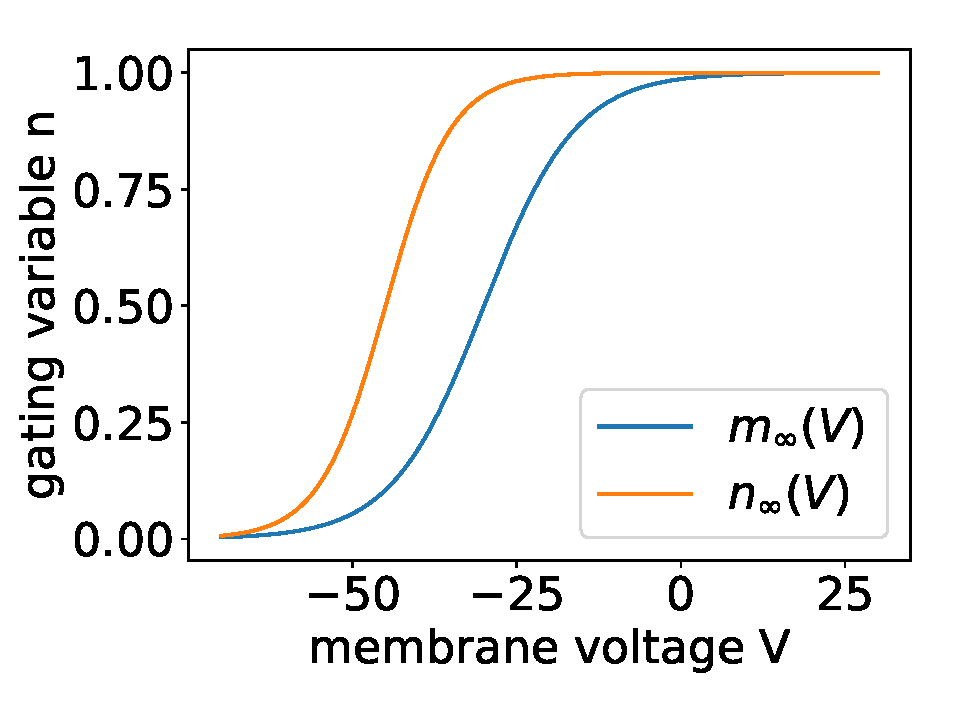
\includegraphics[scale=0.35]{gatinganhopf.pdf}
			\end{figure}
		\end{columns}
	\end{itemize}
\end{adjustwidth}
\end{frame}
\begin{frame}{Phase space}
\begin{columns}[t]
	\column{.5\textwidth}
	\centering
	\vspace{-1cm}
	\begin{figure}
		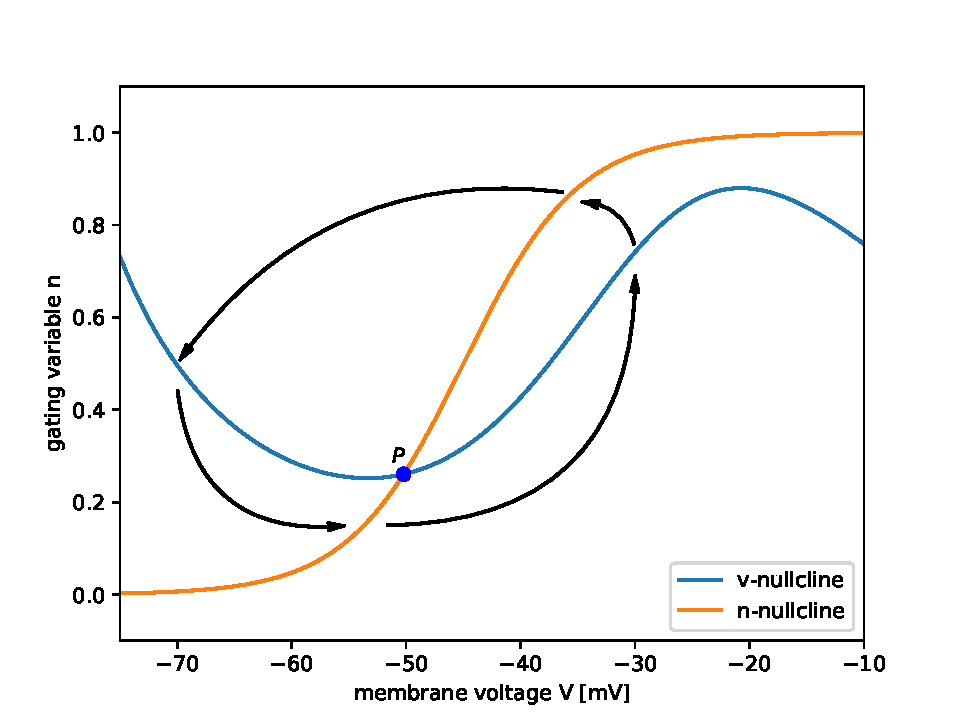
\includegraphics[scale=0.3]{inapikanhopfnc.pdf}
	\end{figure}
	\vspace{-0.5cm}
	\begin{figure}
		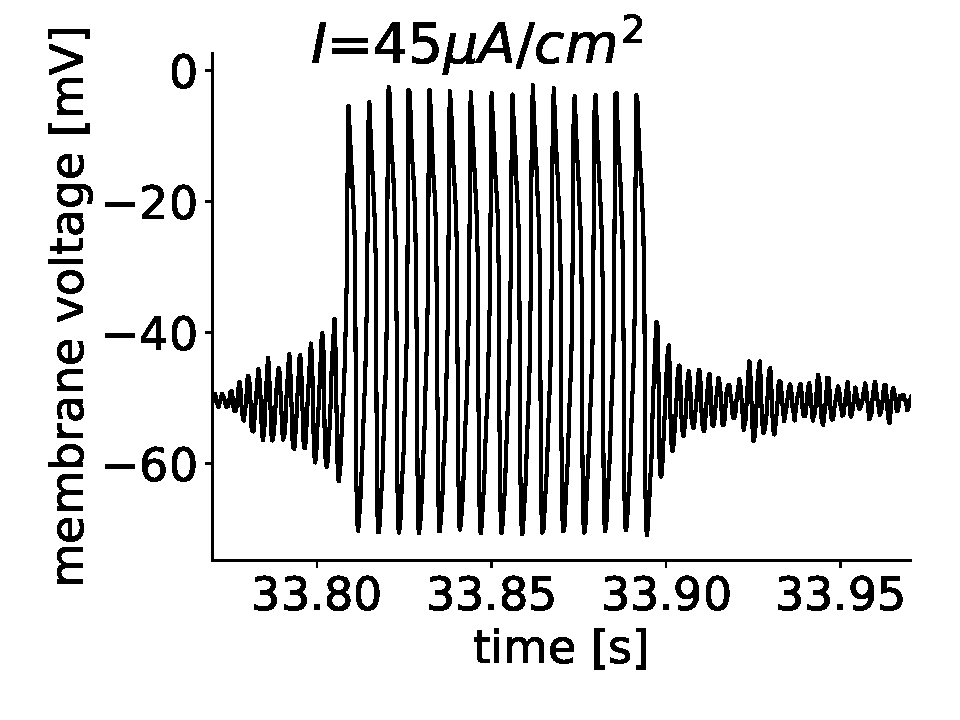
\includegraphics[scale=0.3]{realstateanhopf5sh3.pdf}
	\end{figure}
	\column{.5\textwidth}
	\centering
	\vspace{-1cm}
	\begin{figure}
		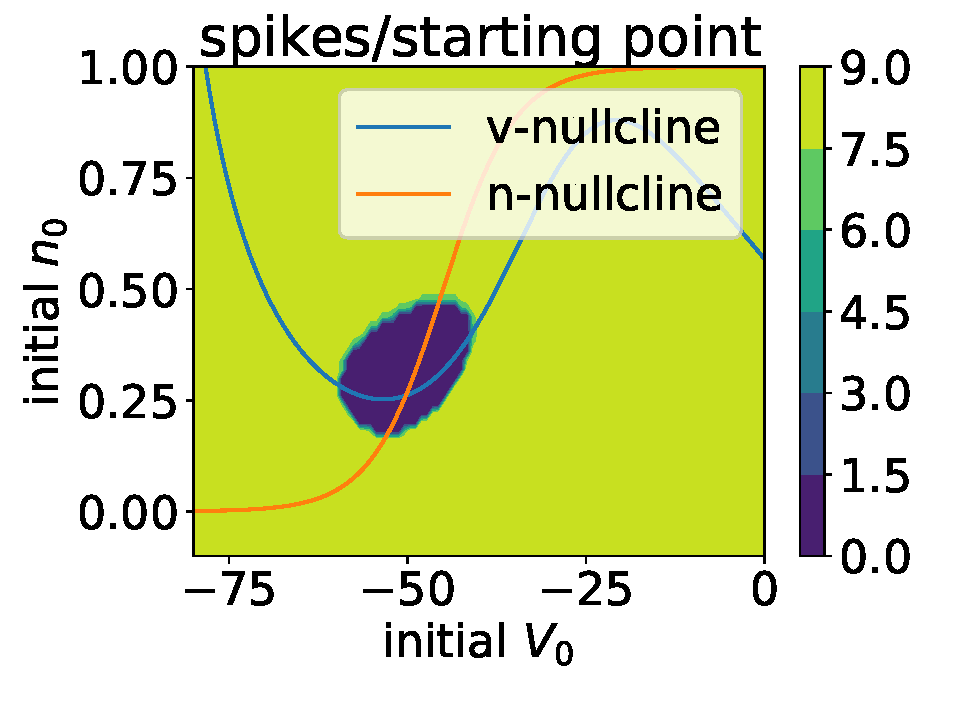
\includegraphics[scale=0.3]{contouranhopfa2sh.pdf}
	\end{figure}\vspace{-0.5cm}
	\begin{figure}
		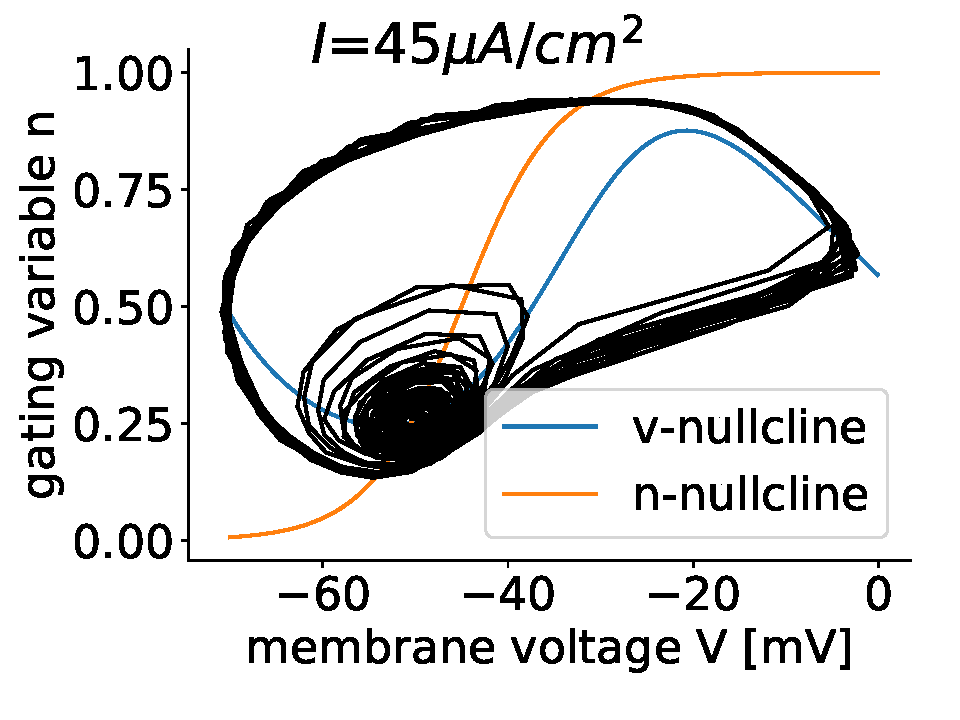
\includegraphics[scale=0.3]{inaprealanhopfreal5psh.pdf}
	\end{figure}
	%\begin{itemize}
	%	\item links oben: rauschinduzierte "Uberg"ange bei $I=0$
	%	\item rechts oben: I=1
	%	\item links unten: I=3
	%\end{itemize}
\end{columns}
\end{frame}
\begin{frame}{Variation of $I$}
\begin{columns}[t]
\column{.5\textwidth}
\vspace{-0.5cm}
\centering
\begin{figure}
	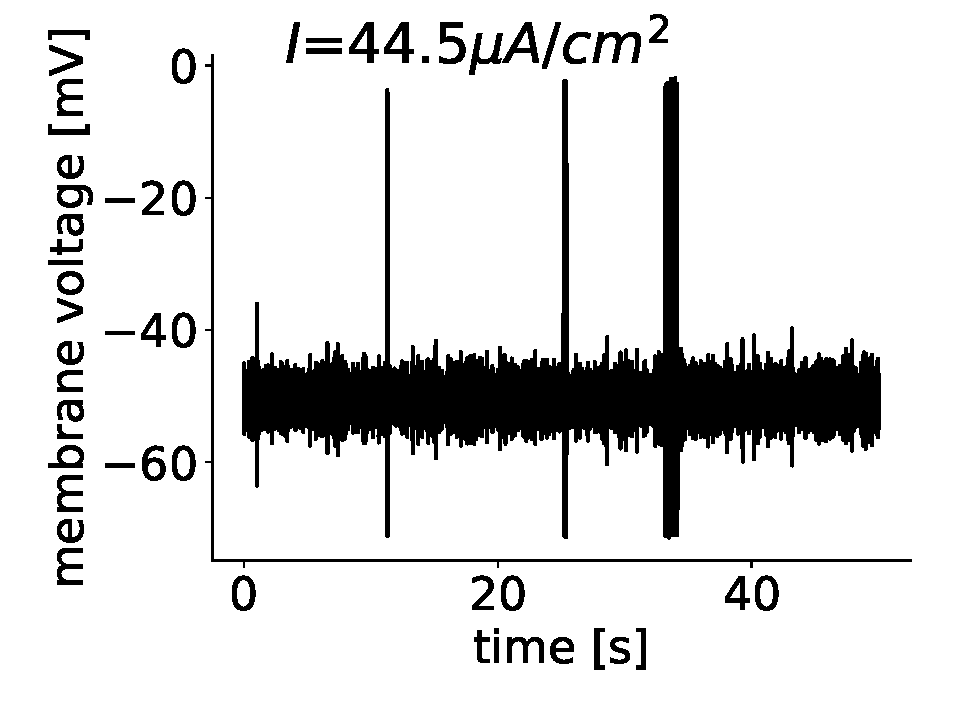
\includegraphics[scale=0.3]{realstateanhopf45full.pdf}
\end{figure}
\vspace{-0.5cm}
\begin{figure}
	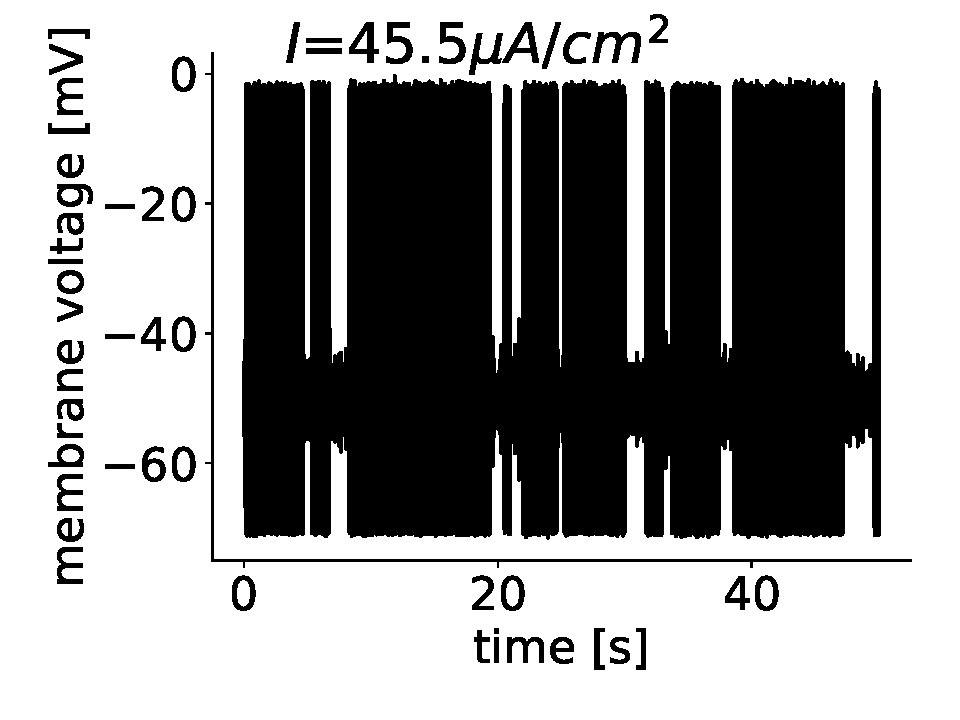
\includegraphics[scale=0.3]{realstateanhopf55full.pdf}
\end{figure}
\column{.5\textwidth}
\vspace{-0.5cm}
\centering
\begin{figure}
	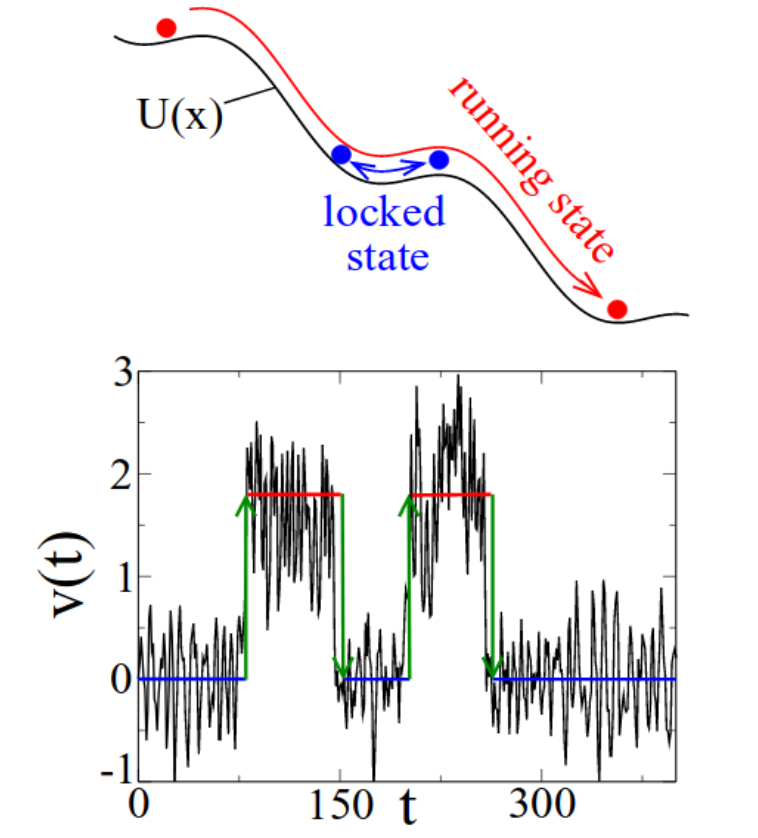
\includegraphics[scale=0.3]{nbpveldyncor2.png}
\end{figure}
\vspace{-8.2cm}
\begin{figure}
	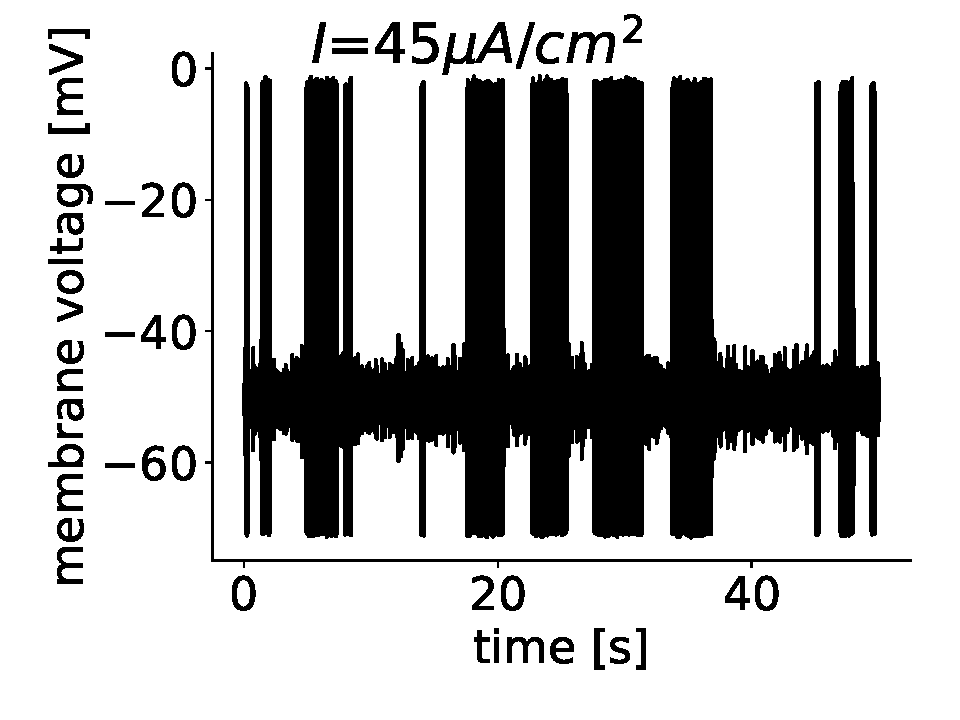
\includegraphics[scale=0.3]{realstateanhopf52full.pdf}
\end{figure}

%\begin{figure}
%	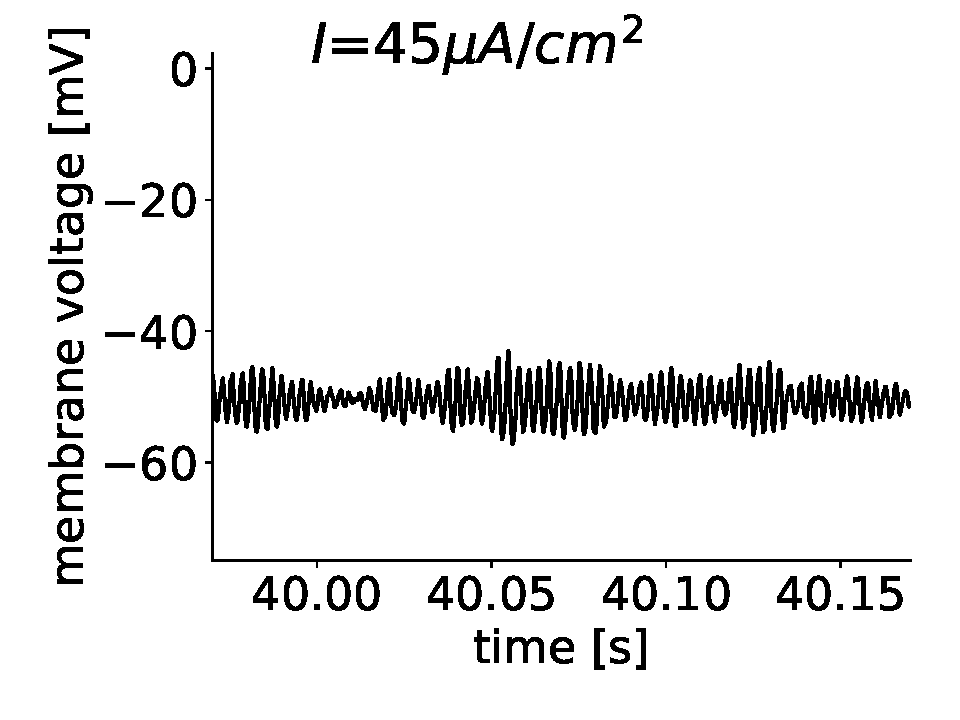
\includegraphics[scale=0.3]{realstateanhopf52sh.pdf}
%\end{figure}

\end{columns}
\end{frame}
\subsection{Simulation}
\begin{frame}{Simulation: firing rate}
\begin{figure}	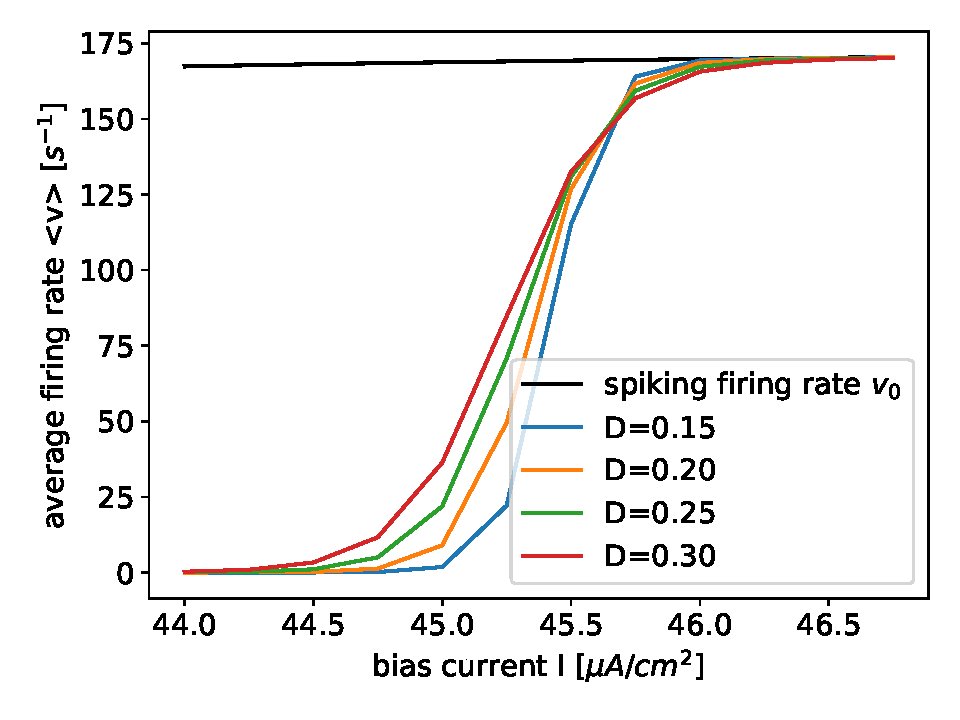
\includegraphics[scale=0.6]{gneur31critsprealanhopf26flogrealanhopf19flog.pdf}
\end{figure}
\end{frame}
\begin{frame}{Simulation: effective diffusion coefficient}
\begin{figure}	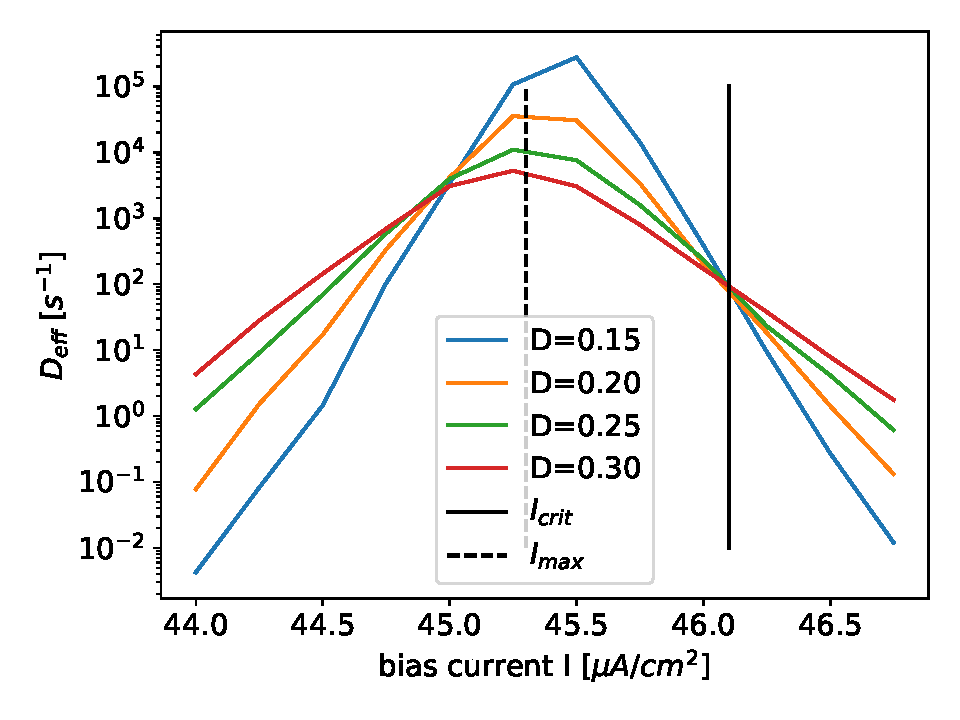
\includegraphics[scale=0.6]{dneur31critrealanhopf26flogrealanhopf19flog.pdf}
\end{figure}
\end{frame}
\begin{frame}{Simulation: Fano factor}
\begin{figure}	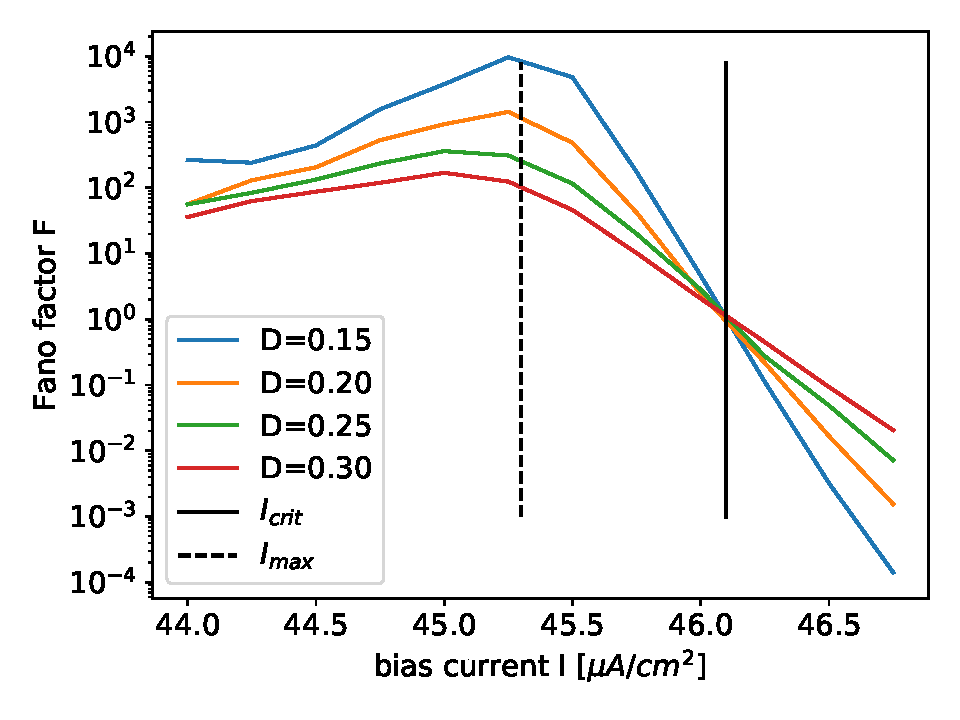
\includegraphics[scale=0.6]{fneur31critrealanhopf26flogrealanhopf19flog.pdf}
\end{figure}
\end{frame}
\subsection{Comparison with other models}
\begin{frame}{Simulation: other models}
\begin{columns}[t]
	\column{.5\textwidth}
	\vspace{-0.5cm}
	\centering
	\begin{figure}
		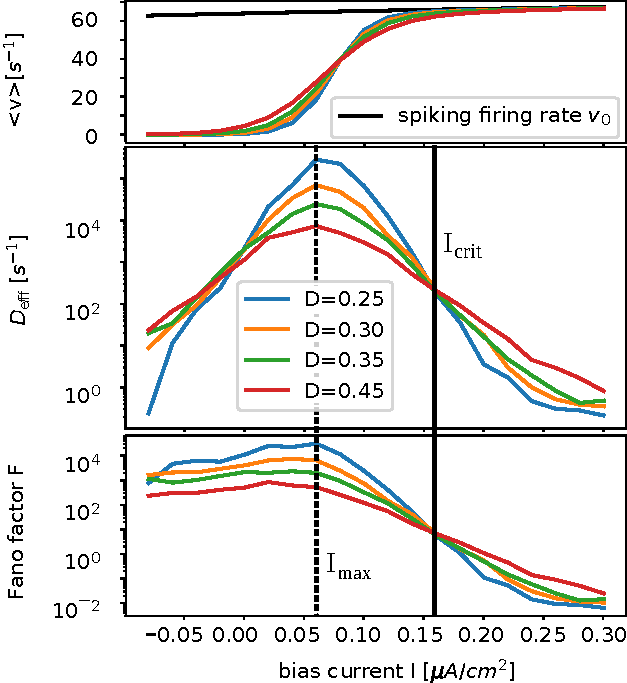
\includegraphics[scale=0.55]{allfast5.pdf}
	\end{figure}
	\column{.5\textwidth}
	\vspace{-0.5cm}
	\centering
	\begin{figure}
	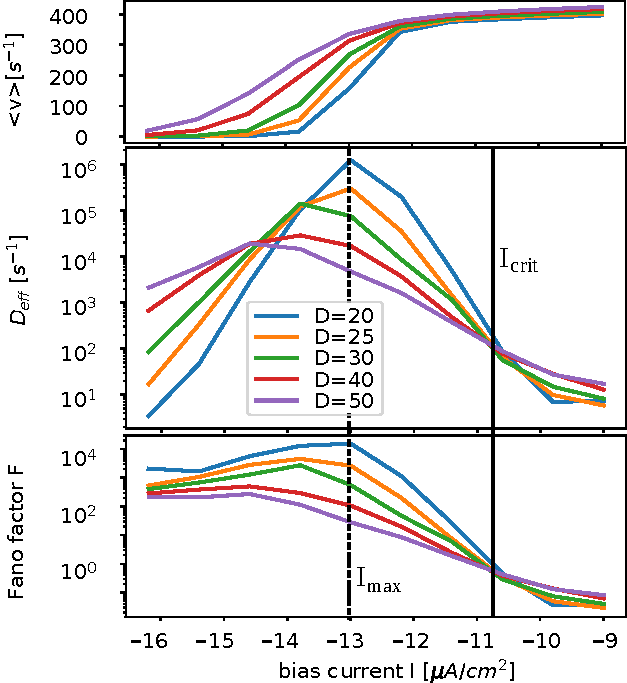
\includegraphics[scale=0.55]{allfastrinzel3.pdf}
	\end{figure}
\end{columns}
\end{frame}
\subsection{Two-state theory}
\begin{frame}{Two-state theory}
\begin{itemize}
	\item \textbf{low noise}: system mostly determined by \textbf{transitions} between states
	\item alternative calculation of $D_{eff}$ using transition rates $r_\pm$\footnotemark[1]
	\begin{align*}
	D_{\text{eff}}=\frac{(\Delta \left<v\right>)^2 r_+r_-}{(r_++r_-)^3}
	\end{align*}
	
	\item fit with \textbf{Arrhenius equation}: effective potential barriers $\Delta U_{\pm}$ and prediction
\end{itemize}
\begin{align*}
r_{\pm}=r_{0,\pm}\text{e}^{-\frac{\Delta U_{\pm}}{D}}
\end{align*}
\footnotetext[1]{C. Van den Broeck, "Taylor dispersion revisited", \textit{Physica A 168}, 1990.}
\end{frame}
\begin{frame}{Comparison with Two-state model: $D_{eff}$}
\begin{figure}	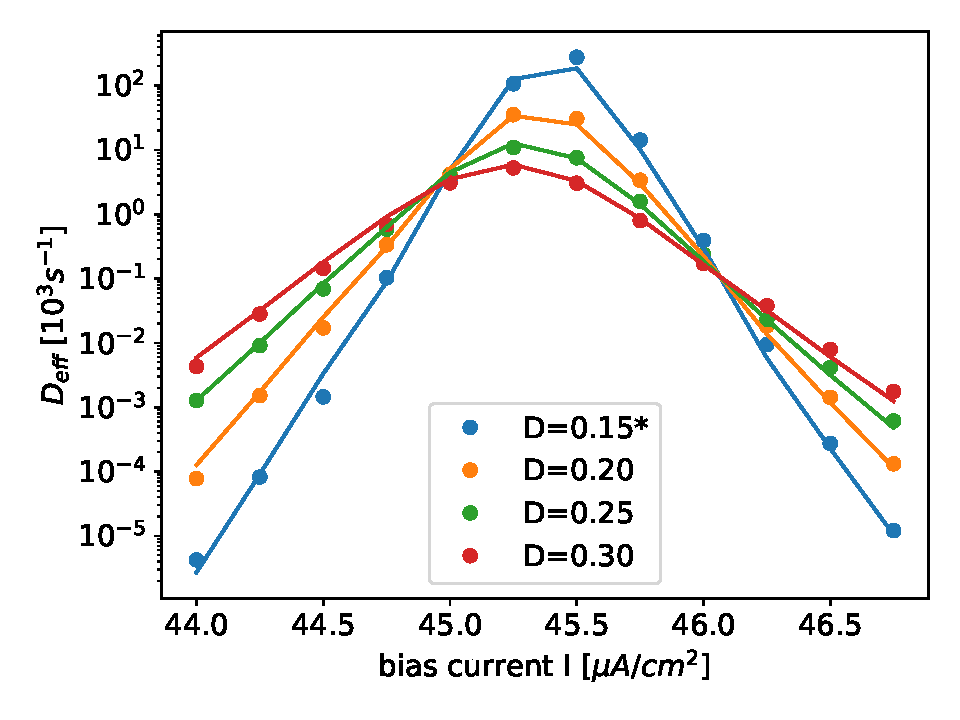
\includegraphics[scale=0.6]{dcompdfpwnew2shdefrealanhopf26flogrealanhopf19flog.pdf}
\end{figure}
\end{frame}
\begin{frame}{Comparison with Two-state model: $F$}
\begin{figure}	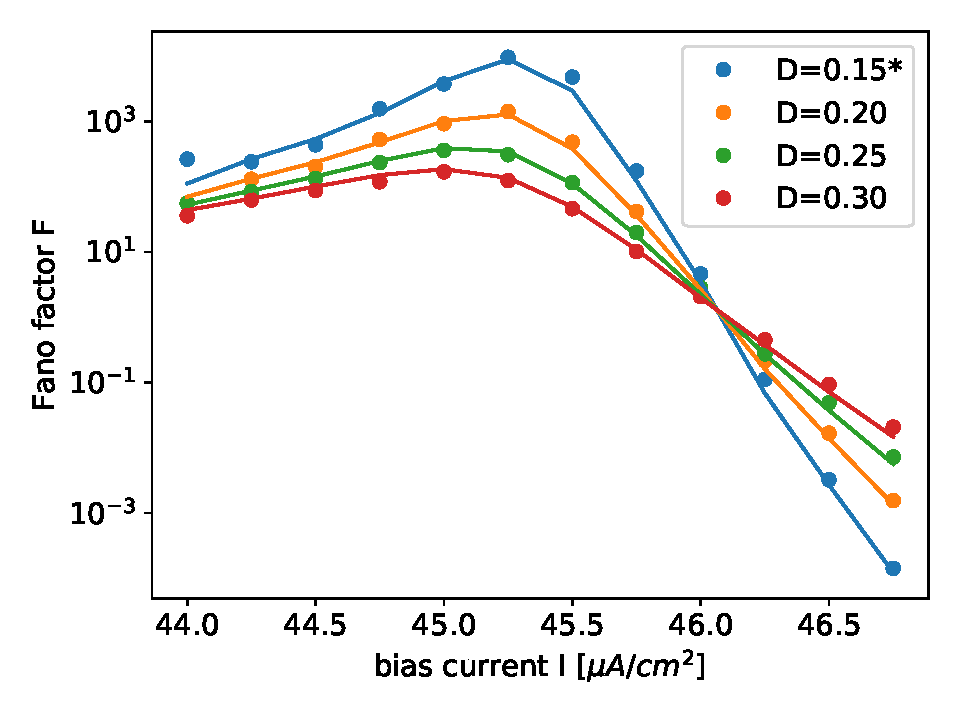
\includegraphics[scale=0.6]{fcompdfpwnew2shdefrealanhopf26flogrealanhopf19flog.pdf}
\end{figure}
\end{frame}
\begin{frame}{Prediction with Two-state model}
\begin{figure}	\includegraphics[scale=0.6]{dcompdfpwnewpred2defrealanhopf19flogrealanhopf11flog.pdf}
\end{figure}
\end{frame}
\section{Signal transmission}
\begin{frame}
\begin{center}
	\Huge{\textcolor{darkred}{Consequences}}
\end{center}
\begin{center}
	\Huge{\textcolor{darkred}{for}}
\end{center}
\begin{center}
	\Huge{\textcolor{darkred}{Signal transmission}}
\end{center}
\end{frame}

\begin{frame}{Measurement of SNR}
\begin{itemize}
	\item System with \textbf{weak+slow} cosine Signal:
	\begin{align*}
	C\dot{V}=f(V,n,t)\rightarrow C\dot{V}=f(V,n,t) + \epsilon\cos(\omega t+\phi)
	\end{align*}
	\item Spectrum from \textbf{Fourier-Trafo} of the $\delta$-Spike-train
	
	\item Signal-to-noise ratio SNR depends on firing rate $\left<v\right>$ and $D_{eff}$\footnotemark[1]:
	\begin{align*}
	SNR=\frac{\Delta S_{peak}}{S_{bg}}=\frac{\epsilon^2T|d\left<v\right>/dI|^2}{8\cdot D_{eff}}
	\end{align*}
			\qquad\qquad\qquad\qquad	$\epsilon$...signal amplitude\\
	\qquad	\qquad	\qquad\qquad	$T$..simulation time\\
	\qquad	\qquad\qquad	\qquad	$I$....bias current
		

\end{itemize}
\footnotetext[1]{L. Gammaitoni et al., "\ Stochastic resonance", \textit{Rev. Mod. Phys. 70}, 1998.}
\end{frame}
%\section{$I_{Na,p}+I_K$-Modell mit Sattel-Knoten Bifurkation}
%	\begin{frame}
%	\begin{center}
%		\Huge{\textcolor{darkred}{$I_{Na,p}+I_K$ Modell}}
%	\end{center}
%	\begin{center}
%		\Huge{\textcolor{darkred}{mit}}
%	\end{center}
%	\begin{center}
%		\Huge{\textcolor{darkred}{Sattel-Knoten-}}
%	\end{center}
%	\begin{center}
%		\Huge{\textcolor{darkred}{Bifurkation}}
%	\end{center}
%\end{frame}
%\begin{frame}{Spektrum mit schwachem periodischen Signal}
%\begin{figure}	\includegraphics[scale=0.62]{specpaper6.pdf}
%\end{figure}
%
%\end{frame}
%\begin{frame}{SNR}
%\begin{figure}	\includegraphics[scale=0.62]{snrealonly2crit2.pdf}
%\end{figure}
%\end{frame}

%\begin{frame}{Vergleich SNR - Theorie}
%\begin{figure}	\includegraphics[scale=0.62]{snrangerealanameasspall.pdf}
%\end{figure}
%\end{frame}



%\begin{frame}{Vergleich SNR - Zwei-Zustands-Theorie}
%\begin{figure}	\includegraphics[scale=0.62]{snrtwostateneurcorsh2.pdf}
%\end{figure}
%\end{frame}
%
%\begin{frame}{Vorhersage mit Zwei-Zustands-Theorie}
%\begin{figure}	\includegraphics[scale=0.62]{snrpredneur.pdf}
%\end{figure}
%\end{frame}
\section{$I_{Na,p}+I_K$ model with Andronov-Hopf Bifurkation}
%\begin{frame}
%\begin{center}
%	\Huge{\textcolor{darkred}{$I_{Na,p}+I_K$ model}}
%\end{center}
%\begin{center}
%	\Huge{\textcolor{darkred}{with}}
%\end{center}
%\begin{center}
%	\Huge{\textcolor{darkred}{Andronov-Hopf-}}
%\end{center}
%\begin{center}
%	\Huge{\textcolor{darkred}{bifurcation}}
%\end{center}
%\end{frame}
\begin{frame}{Frequency Power Spectrum}
\begin{figure}	\includegraphics[scale=0.62]{specanhopf2new.pdf}
\end{figure}
\end{frame}
\begin{frame}{SNR}
\begin{figure}	\includegraphics[scale=0.62]{snranhopfdef.pdf}
\end{figure}
\end{frame}

%\begin{frame}{Vergleich SNR - Theorie}
%\begin{figure}	\includegraphics[scale=0.62]{snrangerealanameasspall.pdf}
%\end{figure}
%\end{frame}
\begin{frame}{SNR: other models}
\begin{columns}[t]
	\column{.5\textwidth}
	\vspace{-0.5cm}
	\centering
	\begin{figure}
		\includegraphics[scale=0.38]{snrsaddlenodedef.pdf}
	\end{figure}
	\column{.5\textwidth}
	\vspace{-0.5cm}
	\centering
	\begin{figure}
		\includegraphics[scale=0.38]{snrinzelonlycritmaxdef.pdf}
	\end{figure}
\end{columns}
\end{frame}
\begin{frame}{Comparison SNR - Two-state theory}
\begin{figure}	\includegraphics[scale=0.62]{snrtwostatecompanhopf7mnofitcrit2def.pdf}
\end{figure}
\end{frame}

\begin{frame}{Prediction with Two-state theory}
\begin{figure}	\includegraphics[scale=0.62]{snranhopfpred.pdf}
\end{figure}
\end{frame}

\section{Summary}
\begin{frame}{Conclusion and outlook}
\begin{itemize}
	\setlength\itemsep{2em}
	\item giant diffusion in multiple models
	$\rightarrow$\textbf{ bistability only requirement}? 
	\item \textbf{critical points} where $D_{eff}$ noise-independent and \textbf{steep changes} of $D_{eff}$ and SNR observed
	\item \textbf{Two-state theory} gives \textbf{good} description
	\item future: experimental investigation of bistable neurons
\end{itemize}
\end{frame}
%\begin{frame}{Conclusion and outlook}
%\begin{center}
%		Questions?
%\end{center}
%
%
%\end{frame}
%\subsection{Zwei-Zustands-Theorie}
%\begin{frame}{Zwei-Zustands-System}
%\begin{itemize}
%	\item geringes Rauschen: Verhalten des Systems durch "Ubergange zwischen Zust"anden bestimmt
%	\item f"ur "Ubergangsraten wird Arrhenius-Gleichung angenommen:
%\end{itemize}
%\begin{align*}
%w_{\pm}=w_{0,\pm}\text{e}^{-\frac{\Delta U_{\pm}}{Q}}
%\end{align*}
%\begin{itemize}
%	\item $w_-$: ruhend zu laufend, $w_+$ umgekehrt, $Q$: Rauschintensit"at
%	\item $D_{\text{eff}}$ aus Raten und $\Delta r=r_+-r_-$:
%\end{itemize}
%\begin{align*}
%D_{\text{eff}}=\frac{(\Delta r)^2 w_+w_-}{(w_++w_-)^3}
%\end{align*}
%\end{frame}
%\begin{frame}{Zwei-Zustands-System}
%\begin{itemize}
%\item gesucht: $F_{crit}$
%\item nahe Schnittpunkt: $D_{\text{eff}}(Q,F)$=$D_{\text{eff}}(F)$
%\item Einsetzen:
%\begin{align*}
%D_{\text{eff}}&=\frac{(\Delta r)^2w_{0,+}w_{0,-}\text{e}^{-\frac{\Delta U_++\Delta U_-}{Q}}}{\left(w_{0,+}\text{e}^{\frac{-\Delta U_+}{Q}}+w_{0,-}\text{e}^{\frac{-\Delta U_-}{Q}}\right)^3}\\&=\frac{(\Delta r)^2w_{0,+}w_{0,-}}{\left(w_{0,+}\text{e}^{-\frac{3\Delta U_+-\Delta U_+-\Delta U_-}{3Q}}+w_{0,-}\text{e}^{-\frac{3\Delta U_--\Delta U_+ -\Delta U_-}{3Q}}\right)^3}\\&=\frac{(\Delta r)^2w_{0,+}w_{0,-}}{\left(w_{0,+}\text{e}^{-\frac{2\Delta U_+-\Delta U_-}{3Q}}+w_{0,-}\text{e}^{-\frac{2\Delta U_--\Delta U_+}{3Q}}\right)^3}
%\end{align*}
%\end{itemize}
%\end{frame}
%\begin{frame}{Zwei-Zustands-System}
%\begin{align*}
%D_{\text{eff}}=\frac{(\Delta r)^2w_{0,+}w_{0,-}}{\left(w_{0,+}\text{e}^{-\frac{2\Delta U_+-\Delta U_-}{3Q}}+w_{0,-}\text{e}^{-\frac{2\Delta U_--\Delta U_+}{3Q}}\right)^3}
%\end{align*}
%\begin{itemize}
%\item Fall 1: $\Delta U_+>\Delta U_-$:
%\begin{align*}
%D_{\text{eff}}\approx\frac{(\Delta r)^2w_{0,+}}{w_{0,-}^2}\text{e}^{-\frac{\Delta U_+-2\Delta U_-}{Q}}
%\end{align*}
%\item bei $\left|\frac{d}{dF}\left(\frac{(\Delta r)^2w_{0,+}}{w_{0,-}^2}\right)/\frac{d}{dF}D_{\text{eff}} \right| \ll 1$:
%\begin{align*}
%\Delta U_+=2\Delta U_-
%\end{align*}
%\item symmetrisches Problem $\rightarrow$ 2. Schnittpunkt bei
%\begin{align*}
%\Delta U_-=2\Delta U_+
%\end{align*}
%\item $\Delta U_\pm =2\Delta U_\mp$
%\end{itemize}
%\end{frame}
%\begin{frame}{Zwei-Zustands-System}
%\begin{itemize}
%\item gesucht: m"ogliche Schnittpunkte im Fano-Faktor
%\begin{align*}
%F=\frac{2D_{\text{eff}}}{r}
%\end{align*}
%\item Mittelwert der Geschwindigkeit:
%\begin{align*}
%r=r_+\frac{w_-}{w_++w_-}
%\end{align*}
%\item Einsetzen der "Ubergangsraten:
%\begin{align*}
%F&=\frac{2r_+w_+}{(w_++w_-)^2}=\frac{2r_+w_{0,+}\text{e}^{-\frac{\Delta U_+}{Q}}}{\left(w_{0,+}\text{e}^{-\frac{\Delta U_+}{Q}}+w_{0,-}\text{e}^{-\frac{\Delta U_-}{Q}}\right)^2}\\
%&=\frac{2r_+w_{0,+}}{\left(w_{0,+}\text{e}^{-\frac{2\Delta U_+-\Delta U_+}{2Q}}+w_{0,-}\text{e}^{-\frac{2\Delta U_--\Delta U_+}{2Q}}\right)^2}
%\end{align*}
%\end{itemize}
%\end{frame}
%\begin{frame}{Zwei-Zustands-System}
%\begin{align*}
%F=\frac{2r_+w_{0,+}}{\left(w_{0,+}\text{e}^{-\frac{2\Delta U_+-\Delta U_+}{2Q}}+w_{0,-}\text{e}^{-\frac{2\Delta U_--\Delta U_+}{2Q}}\right)^2}
%\end{align*}
%\begin{itemize}
%\item $\Delta U_+ > \Delta U_-$:
%\begin{align*}
%F=\frac{2r_+w_{0,+}}{w_{0,-}^2}\text{e}^{-\frac{\Delta U_+-2\Delta U_-}{Q}} \rightarrow \Delta U_+=2\Delta U_-
%\end{align*}
%\item $\Delta U_+ < \Delta U_-$:
%\begin{align*}
%F=\frac{2r_+}{w_{0,+}}\text{e}^{-\frac{\Delta U_+-2\Delta U_+}{Q}} \rightarrow \Delta U_+=0
%\end{align*}
%\item eine Barriere muss verschwinden $\rightarrow$ Rand des G"ultigkeitsbereichs der Zwei-Zustands-Theorie erreicht
%\item rechter Schnittpunkt bleibt erhalten, linker verschiebt sich weiter nach links
%\end{itemize}
%\end{frame}
%\begin{frame}{SNR in Zwei-Zustands-Theorie}
%\begin{itemize}
%\item Ableitung der Feuerrate:
%\begin{align*}
%\frac{dr}{dI}&=\frac{d}{dI}\left(\frac{r_+w_-}{w_++w_-}\right)=\frac{r_+'w_-}{w_++w_-}+\frac{r_+w_-'}{w_++w_-}-\frac{r_+w_-(w_+'+w_-')}{(w_++w_-)^2}\\
%&=\frac{r_+'w_-}{w_++w_-}+\frac{r_+(w_+w_-'-w_-w_+')}{(w_++w_-)^2}
%\end{align*}
%\item Ableitung der "Ubergangsraten:
%\begin{align*}
%w_\pm'=\frac{w_{0,\pm}'}{w_{0,\pm}}w_\pm-\frac{\Delta U_\pm'}{D}w_\pm=\left(\frac{w_{0,\pm}'}{w_{0,\pm}}-\frac{\Delta U_\pm'}{D}\right)w_\pm
%\end{align*}
%\item $r_+'$, $w_{0,\pm}'$ und $\Delta U_\pm'$ numerisch
%\end{itemize}
%\end{frame}
%\begin{frame}{Intervallstatistik}
%\begin{figure}	\includegraphics[scale=0.6]{eqdistajrj2realanhopf19flog354.pdf}
%\end{figure}
%\end{frame}
%\subsection{Zwei-Zustands-Theorie}
%\begin{frame}{Arrhenius-Fit}
%\begin{figure}	\includegraphics[scale=0.6]{arrheniustotbigrealanhopf19flogrealanhopf11flogfit11.pdf}
%\end{figure}
%\end{frame}
%\begin{frame}{Barrieren f"ur verschiedene Str"ome}
%\begin{figure}	\includegraphics[scale=0.6]{barriercompanhopfcritbig.pdf}
%\end{figure}
%\end{frame}
\end{document}

